\documentclass{article}
\usepackage[utf8]{inputenc}
\usepackage[margin=1.75cm]{geometry}
% \usepackage{layouts} % Used to print environment dimensions - used in generating figures
% \usepackage{parskip}
\usepackage{multicol, caption}
\usepackage[table]{xcolor}
\definecolor{l1}{rgb}{0.1068, 0.5480, 0.5020} % Table 1 first row
\definecolor{l2}{rgb}{0.3034, 0.5240, 0.5010} % Table 1 second row
\definecolor{l3}{rgb}{0.5000, 0.5000, 0.5000} % Table 1 third row
\definecolor{l4}{rgb}{0.6966, 0.4760, 0.4990} % Table 1 fourth row
\definecolor{l5}{rgb}{0.8932, 0.4520, 0.4980} % Table 1 fifth row
\usepackage{hyperref}
\usepackage[
backend=biber,
style=apa
]{biblatex}
\addbibresource{bibliography.bib}
\usepackage{svg}
\usepackage{graphicx}

\newenvironment{halffigure}
    {\par\medskip\noindent\minipage{\linewidth}}
    {\endminipage\par\medskip}

\usepackage{amsmath}
\usepackage{amssymb}

% Inversion
\newif\ifinvert
\invertfalse % Set \inverttrue or \invertfalse
\ifinvert % Settings when inverted
\pagecolor[rgb]{0,0,0}
\color[rgb]{1,1,1}
\hypersetup{
    colorlinks=true,
    linkcolor=green,
    citecolor=pink,
    urlcolor=red
}
\else % Settings when normal
\hypersetup{
    colorlinks=true,
    linkcolor=olive,
    citecolor=violet,
    urlcolor=purple
}
\fi

\title{Visualizing Color Space}
\author{Kyle Christopher McDermott}
\date{\today}

\begin{document}

% Title Page
\begin{titlepage}
\maketitle
\thispagestyle{empty} % Removes page number
\end{titlepage}

% Text width is \printinunitsof{in}\prntlen{\textwidth}\\
% Text height is \printinunitsof{in}\prntlen{\textheight}\\
% Line width is \printinunitsof{in}\prntlen{\linewidth}

% ================ SECTION 1 ================

\section{Introduction}

Here are described methods for generating and, in particular, coloring diagrams of color space (chromaticity) and the visible spectrum.  Section \ref{sec:derivation} covers the derivation of the Commission internationale de l'eclairage (CIE) $(x,y)$ chromaticity diagram starting from experimental data collected from human observers, through the derivation of cone (photoreceptor) sensitivities and the color matching functions used to determine chromaticity from light spectra.  Section \ref{sec:color_mixing} uses the chromaticity diagram to illustrate how a few primary colors can be mixed to create a range of colors between, including the sRGB standard which will be used here to determine chromaticity from display color and vice versa.  Section \ref{sec:chromaticity_coloration} presents multiple methods for the coloration of diagrams of chromaticity and of the visible spectrum and the key differences and considerations for selecting among them.  Section \ref{sec:color_temperature} discusses correlated color temperature - relating to black-body radiation and the Planckian locus which is often depicted on chromaticity diagrams.  Finally, Section \ref{sec:color_blindndess} illustrates the theory behind both generating test stimuli for, and filtering images to mimic the effects of, color blindness.

By far the resource used most in the preparation of this document is the excellent database maintained by Andrew Stockman and his colleagues in the Colour \& Vision Research Laboratory at the Institute of Ophthalmology, University College London (\url{http://www.cvrl.org/} or \url{http://cvrl.ucl.ac.uk/}).  The theory, key variables, and tabulated data used both as source and a check on my own computations are there thoughtfully laid out, and links to key pages on their website appear throughout Section \ref{sec:derivation}.

% ================ SECTION 2 ================

\section{Derivation of CIE $(x,y)$ Chromaticity} \label{sec:derivation}

\begin{multicols}{2}

% Text width is \printinunitsof{in}\prntlen{\textwidth}\\
% Line width is \printinunitsof{in}\prntlen{\linewidth}

Typically the color matching functions of CIE 1931 standard (\cite{cie1932commission}) are used to determine the $(x,y)$ chromaticity coordinate from a spectrum of light - doing so for a range of hypothetically purely monochromatic lights results in the “spectrum locus” curve depicted in chromaticity diagrams - and these are based on experiments which presented a relatively small 2$^\circ$ visual angle stimulus to experimental observers (\cite{wright1929re,guild1931colorimetric}).  However, the variables and tabulated data necessary to derive these color matching functions from experimental observations - and to verify my own computations at each step - are more readily available for a larger 10$^\circ$ stimulus (\cite{stiles1959npl}) (which originally contributed to the CIE 1964 standard).  The method detailed here ultimately results in color matching functions for the CIE 170-2 10$^\circ$ Observer standard.  The more typical CIE 1931 2$^\circ$ Observer standard color matching functions will be used in later sections primarily because the sRGB primaries are defined in that space.  As will be illustrated, the 2$^\circ$ and 10$^\circ$ chromaticity diagrams are similar enough to make the distinction important only for narrowly defined circumstances (i.e. experiments probing human vision).

\subsection{Color Matching Experiment} % 2.1

Stiles \& Burch presented in 1959 data from 49 individual observers (including 4 experimenters who are represented twice for a total of 53 observations across two similar conditions) using a 10$^\circ$ Stimulus (\cite{stiles1959npl}).  They also presented data from 10 observers for a 2$^\circ$ stimulus, but this has been deemed too few from which to build a “standard observer”.  The Color \& Vision Research Laboratory have made the data available here (file download \href{http://www.cvrl.org/database/data/sb_individual/SB10_corrected_indiv_CMFs.xls}{link}); these are “corrected data” (see \href{http://www.cvrl.org/database/text/sb_individual/sb10_individual.htm}{here} (\cite{stiles1958average})).

\subsubsection{Stimuli \& Procedure} % 2.1.1

The experiment presented observers with a circular stimulus 10$^\circ$ in diameter, bisected vertically.  On the "test" side were presented a range of narrow-band lights from 14,000 $cm^{-1}$ to 25,500 $cm^{-1}$ (roughly 714 $nm$ to 392 $nm$, note the reversed order as the units are inverses of each other).  On the other, "match" side was a mixture of (up to) three “primary” lights at 15,500 $cm^{-1}$ (roughly 645 $nm$, and reddish), 19,000 $cm^{-1}$ (roughly 526 $nm$, and greenish), and 22,500 $cm^{-1}$ (roughly 444 $nm$, and bluish); the experimental data are “transformed” from the actual, physical values of 15,418 $cm^{-1}$, 18,997 $cm^{-1}$, and 22,456 $cm^{-1}$, respectively.  Observers’ task was to adjust the intensity of the three primary lights on one side to match the single light on the other side.

As will be illustrated later, it is not always possible to mix three primaries in this way to create a match if the test stimulus is outside the range of colors achievable by a mixing of those primaries.  Therefore the experimenters allowed the primaries to be adjusted to “negative” intensities - this meant that instead of adding the primary to the "match" side, it was instead added to the "test" side.  Therefore, when one of the primaries was adjusted to a negative intensity, observers were adjusting the appearance of both sides of the stimulus to match them.

\subsubsection{Data Visualization} % 2.1.2

\begin{figure*} % Figure 1
    \ifinvert
        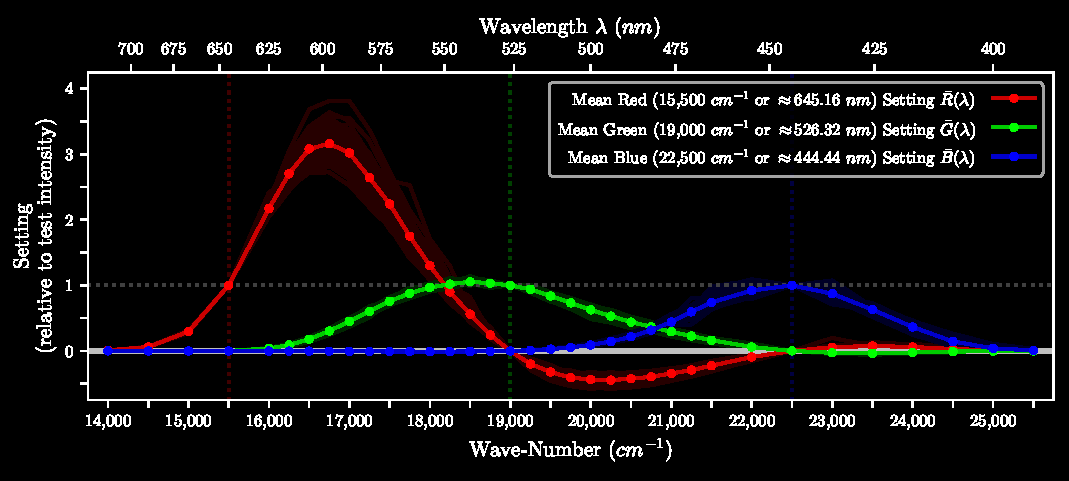
\includegraphics{../images/figure_01_color_matching_experiment_data_inverted.pdf}
    \else
        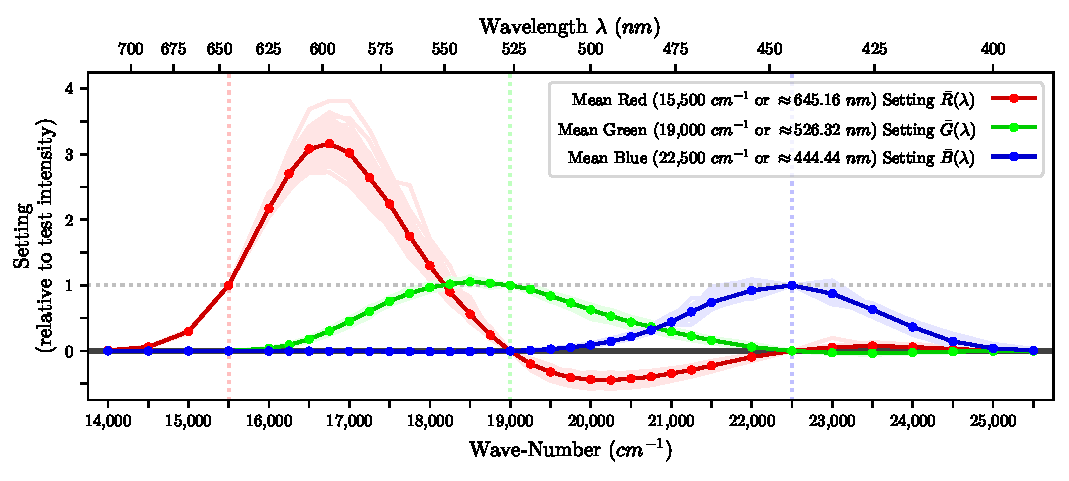
\includegraphics{../images/figure_01_color_matching_experiment_data.pdf}
    \fi
    \caption{Individual (faded) and average (bold) settings of the red, green, and blue primary lights relative to the test light intensity plotted across all test light wave-numbers.  Positive settings indicate primary lights added together on the "match" side of the stimulus.  Negative settings indicate primary lights instead added to the "test" side of the stimulus along with the test light.  Where horizontal and vertical dotted lines cross, no settings were recorded (note there is zero individual variability at these points); instead it was presumed that each primary would exactly match itself in isolation.  Note that the step size between test lights is larger below 16,000 $cm^{-1}$ and above 21,500 $cm^{-1}$. IMAGE LINK, CODE LINK}\label{fig:color_matching_experiment_data}
\end{figure*}

Figure \ref{fig:color_matching_experiment_data} plots the 53 individual traces of observers' settings as well as the average (in bold).  The original data are given in wave-number ($cm^{-1}$), however we will generally be using wavelength ($nm$) in our formulations and assign the symbol lambda ($\lambda$) to it.  The experimental average settings for the red, green, and blue primaries - as functions of wavelength $\lambda$ - are symbolized by $\bar{R}(\lambda)$, $\bar{G}(\lambda)$, and $\bar{B}(\lambda)$, respectively.

\begin{halffigure} % Figure 2
    \ifinvert
        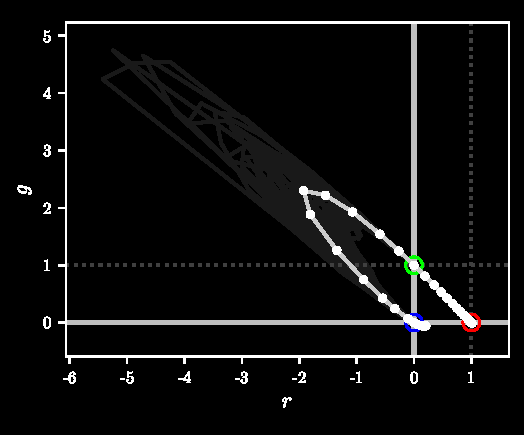
\includegraphics{../images/figure_02_color_matching_experiment_chromaticity_inverted.pdf}
    \else
        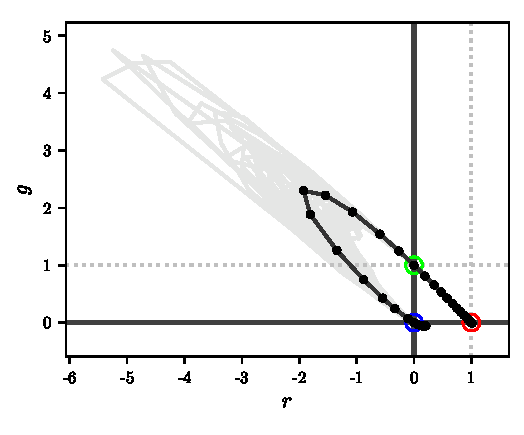
\includegraphics{../images/figure_02_color_matching_experiment_chromaticity.pdf}
    \fi
    \captionof{figure}{Individual (faded) and average (bold) settings converted to experimental chromaticity.  Note that the settings between 19,000 $cm^{-1}$ (green) and 22,500 $cm^{-1}$ (blue) where the red setting is negative (see Figure \ref{fig:color_matching_experiment_data}) extend up and left relatively far, and that the individual variability here is also magnified. IMAGE LINK, CODE LINK}\label{fig:color_matching_experiment_chromaticity}
\end{halffigure}

The red, green, and blue primary settings can be reduced to two values to form a chromaticity coordinate in the experimental chromaticity space.  The chromaticity coordinates - as functions of wavelength $\lambda$ - $\bar{r}(\lambda)$ and $\bar{g}(\lambda)$ are given by:

\begin{equation} % Equation 1
    \begin{aligned}
        \bar{r}(\lambda)&=\frac{\bar{R}(\lambda)}{\bar{R}(\lambda)+\bar{G}(\lambda)+\bar{B}(\lambda)}\\
        \bar{g}(\lambda)&=\frac{\bar{G}(\lambda)}{\bar{R}(\lambda)+\bar{G}(\lambda)+\bar{B}(\lambda)}
    \end{aligned}
\end{equation}

Figure \ref{fig:color_matching_experiment_chromaticity} plots the settings from Figure \ref{fig:color_matching_experiment_data} converted into this experimental chromaticity space.  Note that the individual variability among test wave-numbers between the green and blue primaries are relatively large; bear this in mind when presented with the different chromaticity diagrams of the CIE standards presented later (see Figure \ref{fig:chromaticity_spaces}).

\begin{figure*} % Figure 3
    \ifinvert
        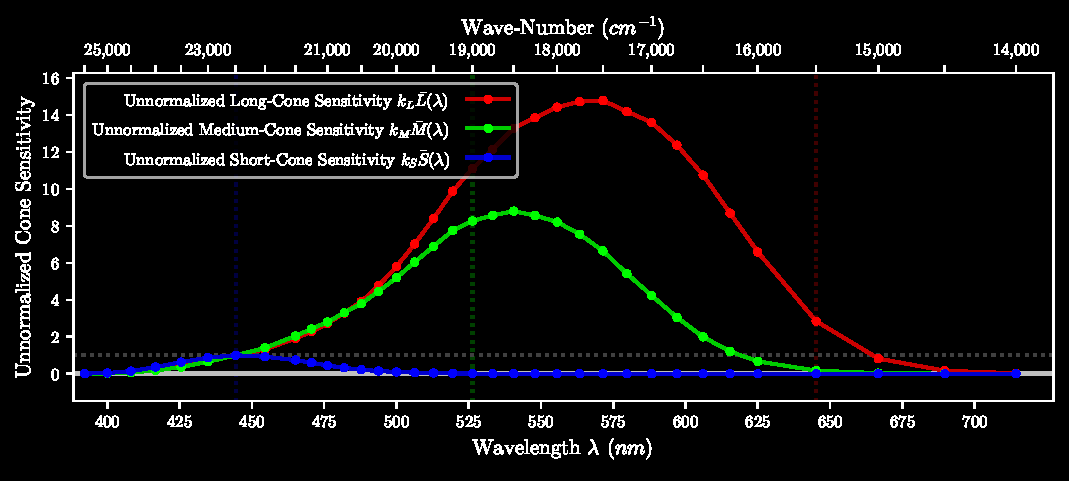
\includegraphics{../images/figure_03_unnormalized_cone_fundamentals_inverted.pdf}
    \else
        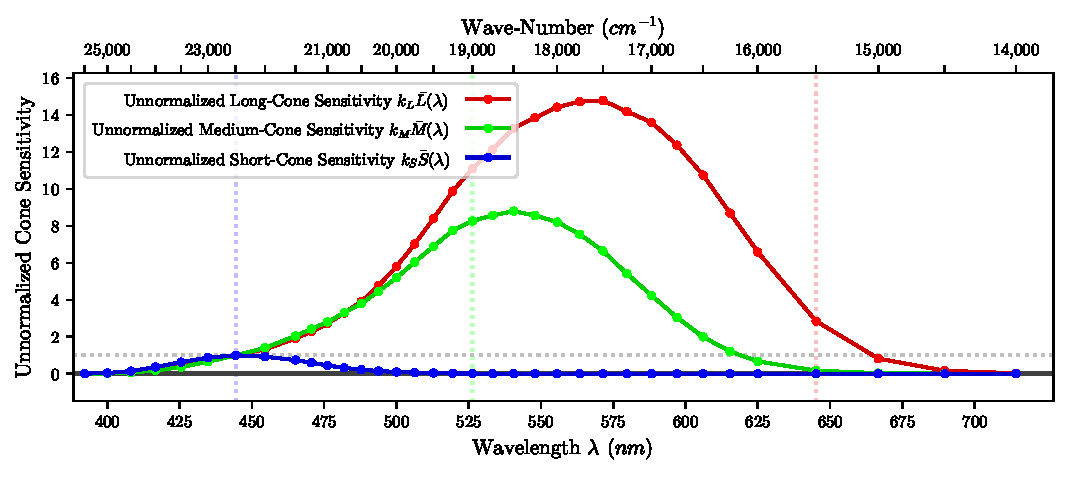
\includegraphics{../images/figure_03_unnormalized_cone_fundamentals.pdf}
    \fi
    \caption{Unnormalized cone fundamentals transformed from color matching experiment mean settings using Equation \ref{eq:cone_fundamental_linear_transformation}.  Dashed vertical lines indicate the wavelengths of the experimental primary lights; note that all three fundamentals pass through $1.0$ at the wavelength corresponding to the experimental blue primary.  IMAGE LINK, CODE LINK}\label{fig:unnormalized_cone_fundamentals}
\end{figure*}

\subsubsection{Links} % 2.1.3

\begin{itemize}
    \item Colour \& Vision Research Laboratory
    \begin{itemize}
        \item \href{http://www.cvrl.org/stilesburch10_ind.htm}{Stiles \& Burch individual 10$^\circ$ color matching data}
    \end{itemize}
    \item Figure Images
    \begin{itemize}
        \item FIGURE 1 LIGHT AND DARK SVG
        \item FIGURE 2 LIGHT AND DARK SVG
    \end{itemize}
    \item GitHub Scripts
    \begin{itemize}
        \item DATA INGESTION OF INDIVIDUAL AND MEAN DATA
        \item FIGURE GENERATION FOR FIGURES 1 \& 2
    \end{itemize}
\end{itemize}

\subsection{Conversion to Cone Sensitivities} % 2.2

In order to get from the color matching experimental data described above to the color matching \textit{functions} that will define the color spaces we wish to visualize we need to go through the "cone fundamentals" which describe the relative sensitivity to different wavelengths of light of the three types of cone photoreceptors.  The experiments used to measure the sensitivities of the different cone types will not be explored in detail, however the articles that describe these experiments present the necessary conversion constants to transform the matching experiment data into the cone fundamentals (and later to transform the cone fundamentals into the color matching functions).

\begin{figure*} % Figure 4
    \ifinvert
        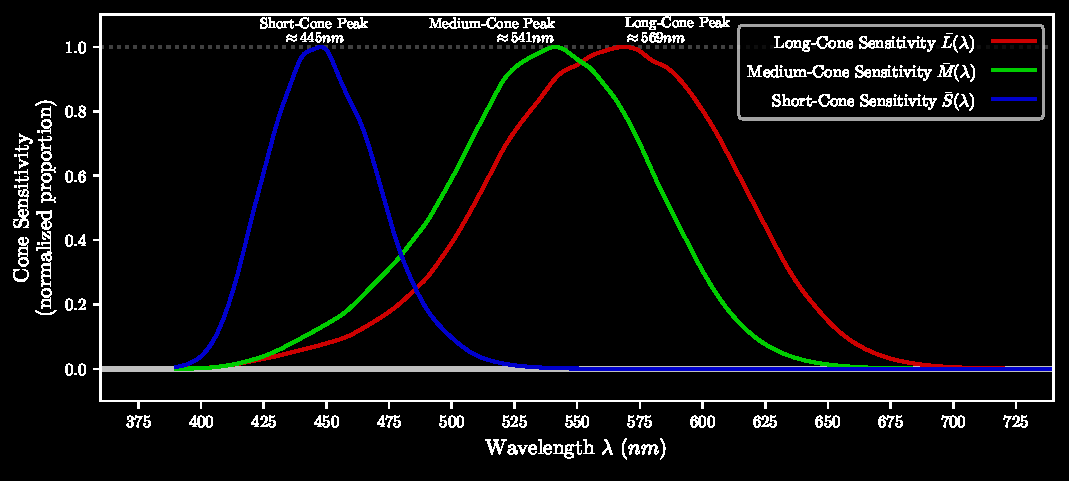
\includegraphics{../images/figure_04_cone_fundamentals_inverted.pdf}
    \else
        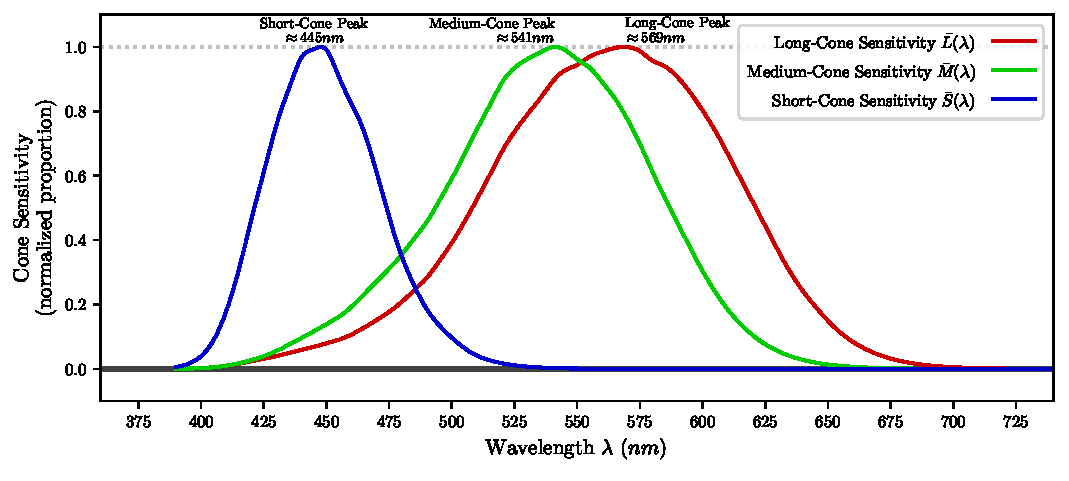
\includegraphics{../images/figure_04_cone_fundamentals.pdf}
    \fi
    \caption{Normalized, smoothed cone fundamentals.  The approximate peak of each cone's sensitivity curve is annotated.  IMAGE LINK, CODE LINK}\label{fig:cone_fundamentals}
\end{figure*}

\subsubsection{Conversion Equations} % 2.2.1

The cone fundamentals are expressed as linear combinations of the three (average) settings for the red, green, and blue primaries from the color matching experiment:

\begin{equation} % Equation 2
    \begin{aligned}
        L_R\bar{R}(\lambda)+L_G\bar{G}(\lambda)+L_B\bar{B}(\lambda)&=\bar{L}(\lambda)\\
        M_R\bar{R}(\lambda)+M_G\bar{G}(\lambda)+M_B\bar{B}(\lambda)&=\bar{M}(\lambda)\\
        S_R\bar{R}(\lambda)+S_G\bar{G}(\lambda)+S_B\bar{B}(\lambda)&=\bar{S}(\lambda)
    \end{aligned}
\end{equation}

where $\bar{L}(\lambda)$, $\bar{M}(\lambda)$, and $\bar{S}(\lambda)$ are the sensitivities of the long-, medium-, and short-wavelength-sensitive cones, respectively.  The coefficients $L_R$, $L_G$, ..., $S_G$, and $S_B$ are to be determined experimentally.

The above linear combinations can be expressed as a linear transformation:

\begin{equation} % Equation 3
    \begin{bmatrix}
        L_R&L_G&L_B\\
        M_R&M_G&M_B\\
        S_R&S_G&S_B
    \end{bmatrix}\begin{bmatrix}
        \bar{R}(\lambda)\\
        \bar{G}(\lambda)\\
        \bar{B}(\lambda)
    \end{bmatrix}=\begin{bmatrix}
        \bar{L}(\lambda)\\
        \bar{M}(\lambda)\\
        \bar{S}(\lambda)
    \end{bmatrix}
\end{equation}

At this stage there are nine coefficients to find, however there are two things that can reduce this number: first, we will assert that we don't need to find the absolute sensitivities of the different cone types - we only wish to get the shape of the functions, but will normalize them to get \textit{relative} sensitivity only - and second, we will assert that the short-wavelength-sensitive cones are completely insensitive to the red primary light used in the color matching experiment.  Arbitrarily choosing the coefficients for the blue primary light, we use them to define three normalization constants $k$ as:

\begin{equation}\label{eq:cone_fundamental_normalization_constants_symbolic} % Equation 4
    \begin{aligned}
        k_L&=\frac{1}{L_B}\\
        k_M&=\frac{1}{M_B}\\
        k_S&=\frac{1}{S_B}
    \end{aligned}
\end{equation}

the values of which will be determined later so as to independently make the maximum of each cone sensitivity equal to $1.0$.  Factoring these into the linear transformation gives:

\begin{equation}\label{eq:cone_fundamental_linear_transformation_symbolic_simplified} % Equation 5
    \begin{bmatrix}
        \frac{L_R}{L_B}&\frac{L_G}{L_B}&1\\
        \frac{M_R}{M_B}&\frac{M_G}{M_B}&1\\
        0&\frac{S_G}{S_B}&1
    \end{bmatrix}\begin{bmatrix}
        \bar{R}(\lambda)\\
        \bar{G}(\lambda)\\
        \bar{B}(\lambda)
    \end{bmatrix}=\begin{bmatrix}
        k_L\bar{L}(\lambda)\\
        k_M\bar{M}(\lambda)\\
        k_S\bar{S}(\lambda)
    \end{bmatrix}
\end{equation}

and now there are only five coefficients to find.

\subsubsection{Constants from Experimentation} % 2.2.2

By comparing the sensitivity of observers who possess only short-wavelength-sensitive cones (\textit{s}-cone monochromats) to typical trichromats the sensitivity of \textit{s}-cones to various wavelengths of light was determined and the coefficient $\frac{S_G}{S_B}$ was estimated to be $0.010600$ (\cite{stockman1999spectral}).  Color-blind observers with missing \textit{m}- or \textit{l}-cones were compared to trichromats to derive the remaining coefficients: $\frac{L_R}{L_B}=2.846201$, $\frac{L_G}{L_B}=11.092490$, $\frac{M_R}{M_B}=0.168926$, and $\frac{M_G}{M_B}=8.265895$ (\cite{stockman2000spectral}), filling out the linear transformation:

\begin{equation}\label{eq:cone_fundamental_linear_transformation} % Equation 6
    \begin{bmatrix}
        2.846201&11.092490&1\\
        0.168926&8.265895&1\\
        0&0.010600&1
    \end{bmatrix}\begin{bmatrix}
        \bar{R}(\lambda)\\
        \bar{G}(\lambda)\\
        \bar{B}(\lambda)
    \end{bmatrix}=\begin{bmatrix}
        k_L\bar{L}(\lambda)\\
        k_M\bar{M}(\lambda)\\
        k_S\bar{S}(\lambda)
    \end{bmatrix}
\end{equation}

Passing the mean color matching experiment settings through this linear transformation gives us the correct shapes of the cone fundamentals, however their relative scale is still arbitrary (see Figure \ref{fig:unnormalized_cone_fundamentals}).  All three series pass through a value of $1.0$ where the wavelength of light matches the blue experimental primary simply because of the method used to define the constants $k$.

\subsubsection{Normalization} % 2.2.3

The Colour \& Vision Research Laboratory does not list their computed normalization constants $k$, but the procedure is straightforward and we can check our work with their tabulated values for the normalized cone sensitivities.  Using quadratic spline interpolation to smooth out the unnormalized cone fundamentals in Figure \ref{fig:unnormalized_cone_fundamentals}, the peak sensitivities for the long-, medium-, and short-wavelength sensitive cones are $k_L\approx14.831370$, $k_M\approx8.797703$, and $k_S\approx1.001009$, respectively (at $569 nm$, $541 nm$, and $445 nm$, respectively) (CODE LINK).  Using Equation \ref{eq:cone_fundamental_normalization_constants_symbolic} to solve for $L_B$, $M_B$, and $S_B$ and factoring into the linear transformation in Equation \ref{eq:cone_fundamental_linear_transformation_symbolic_simplified} we now have the linear transformation to convert from the color matching experiment mean settings into \textit{normalized} cone fundamentals:

\begin{equation} % Equation 7
    \begin{bmatrix}
        0.191904&0.747907&0.067425\\
        0.019201&0.939552&0.113666\\
        0&0.010589&0.998992
    \end{bmatrix}\begin{bmatrix}
        \bar{R}(\lambda)\\
        \bar{G}(\lambda)\\
        \bar{B}(\lambda)
    \end{bmatrix}=\begin{bmatrix}
        \bar{L}(\lambda)\\
        \bar{M}(\lambda)\\
        \bar{S}(\lambda)
    \end{bmatrix}
\end{equation}

Figure \ref{fig:cone_fundamentals} shows the resulting normalized cone fundamentals smoothed by interpolation.

\subsubsection{Links} % 2.2.4

\begin{itemize}
    \item Article Full Text
    \begin{itemize}
        \item \cite{stockman1999spectral} - \href{https://www.sciencedirect.com/science/article/pii/S0042698998002259}{article page}
        \item \cite{stockman2000spectral} - \href{https://www.sciencedirect.com/science/article/pii/S0042698900000213}{article page}
    \end{itemize}
    \item Colour \& Vision Research Laboratory
    \begin{itemize}
        \item \href{http://www.cvrl.org/cones.htm}{Cone Fundamentals Data Sets}
        \item \href{http://www.cvrl.org/database/text/cones/ss10.htm}{10$^\circ$ Cone Fundamentals Information}
    \end{itemize}
    \item Figure Images
    \begin{itemize}
        \item FIGURE 3 LIGHT AND DARK SVG
        \item FIGURE 4 LIGHT AND DARK SVG
    \end{itemize}
    \item GitHub Scripts
    \begin{itemize}
        \item DATA INGESTION OF CONE FUNDAMENTALS
        \item ESTIMATION OF NORMALIZATION CONSTANTS
        \item FIGURE GENERATION FOR FIGURES 3 \& 4
    \end{itemize}
\end{itemize}

\subsection{Color Matching Functions} % 2.3

The CIE color matching functions, and the resulting chromaticity diagram, do not directly represent the results of a color matching \textit{experiment}.  The chromaticity coordinates $x$ and $y$ do not represent primary lights of any physically realizable spectrum.  Whereas chromaticities along the vertical ($r=0$) and horizontal ($g=0$) axes in the $(r,g)$ chromaticity diagram depicted in Figure \ref{fig:experiment_chromaticity} represent actual colors within the bounds of those that can be achieved by mixing the primaries together, the vertical and horizontal axes of the $(x,y)$ chromaticity diagram are outside of the spectrum locus and the realm of possible physical colors.  Part of the reasoning behind the construction of the $(x,y)$ chromaticity diagram is, in fact, to have all possible physical colors fall within the bounding triangle of $0$ to $1$ on the two axes and the line $x+y=1$.

\begin{halffigure} % Figure 5
    \ifinvert
        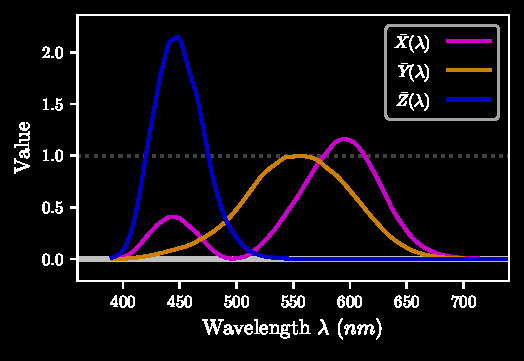
\includegraphics{../images/figure_05_color_matching_functions_inverted.pdf}
    \else
        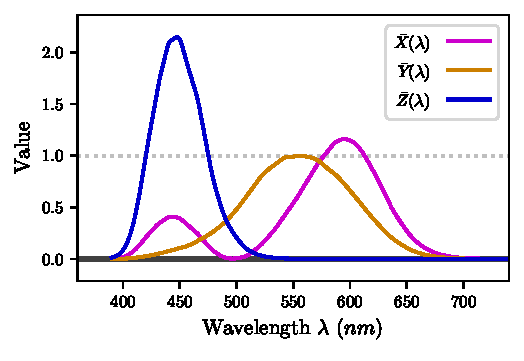
\includegraphics{../images/figure_05_color_matching_functions.pdf}
    \fi
    \captionof{figure}{CIE 170-2 10$^\circ$ color matching functions transformed from the 10$^\circ$ cone fundamentals.  Note that $\bar{Y}(\lambda)$ peaks at $1.0$ and the integrated area under all three functions are equal to each other. IMAGE LINK, CODE LINK}\label{fig:color_matching_functions}
\end{halffigure}

The color matching functions can each be expressed as a linear combination of the three cone fundamentals:

\begin{equation} % Equation 8
    \begin{aligned}
        X_L\bar{L}(\lambda)+X_M\bar{M}(\lambda)+X_S\bar{S}(\lambda)&=\bar{X}(\lambda)\\
        Y_L\bar{L}(\lambda)+Y_M\bar{M}(\lambda)+Y_S\bar{S}(\lambda)&=\bar{Y}(\lambda)\\
        Z_L\bar{L}(\lambda)+Z_M\bar{M}(\lambda)+Z_S\bar{S}(\lambda)&=\bar{Z}(\lambda)
    \end{aligned}
\end{equation}

where $\bar{X}(\lambda)$, $\bar{Y}(\lambda)$, and $\bar{Z}(\lambda)$ are the color matching functions.  The letters don't correspond to color or cone type, and are thus arbitrarily chosen.  The coefficients $X_L$, $X_M$, ..., $Z_M$, and $Z_S$ need to be determined.  As before, we will express the above set linear of combinations as a linear transformation:

\begin{equation} % Equation 9
    \begin{bmatrix}
        X_L&X_M&X_S\\
        Y_L&Y_M&Y_S\\
        Z_L&Z_M&Z_S
    \end{bmatrix}\begin{bmatrix}
        \bar{L}(\lambda)\\
        \bar{M}(\lambda)\\
        \bar{S}(\lambda)
    \end{bmatrix}=\begin{bmatrix}
        \bar{X}(\lambda)\\
        \bar{Y}(\lambda)\\
        \bar{Z}(\lambda)
    \end{bmatrix}
\end{equation}

\subsubsection{Luminous Efficiency} % 2.3.1

The second color matching function $\bar{Y}(\lambda)$ is constructed to represent luminance, or perceived brightness.  The perceived brightness of lights of different wavelengths is expressed by a luminous efficiency function which depends, among other things, on the state of adaptation of the visual system being measured experimentally.  The perception of brightness is driven by the long- and medium-wavelength-sensitive cones, so the coefficient $Y_S=0$ and the short-wavelength-sensitive cone activation will not impact $\bar{Y}(\lambda)$.  The ratio of long- to medium-wavelength -sensitive cone contribution to luminous efficiency under normal daylight adaptation conditions was determined experimentally to be $\approx1.981377$ (\cite{sharpe2011luminous}):

\begin{equation} % Equation 10
    1.981377\bar{L}(\lambda)+\bar{M}(\lambda)=V^*_{D65}(\lambda)
\end{equation}

where $V^*_{D65}$ is luminous efficiency when the visual system is adapted to standard illuminant $D65$ (normal daylight with a correlated color temperature of approximately $6,500K$).  The color matching function $\bar{Y}(\lambda)$ is further constrained to peak at $1.0$ and so, while maintaining the above ratio, its linear combination is:

\begin{equation} % Equation 11
    0.692839\bar{L}(\lambda)+0.349676\bar{M}(\lambda)=\bar{Y}(\lambda)
\end{equation}

\subsubsection{Remaining Functions} % 2.3.2

The third color matching function $\bar{Z}(\lambda)$ depends only on the activation of the short-wavelength-sensitive cone, so $Z_L=0$ and $Z_M=0$.  All three color matching functions have the same integral (area under the curve) and so the linear combination for the third function is:

\begin{equation} % Equation 12
    2.146879\bar{S}(\lambda)=\bar{Z}(\lambda)
\end{equation}

so that its area matches that under $\bar{Y}(\lambda)$.

Of the three color matching functions $\bar{X}(\lambda)$ bears the least resemblance to any physiological feature of the visual system - in fact, it has two peaks.  This function is constructed to give the resulting chromaticity diagram some of its features, visualized later, but in short the realm of physical colors is contained within the triangular area described earlier and to fill that area reasonably efficiently.  The following linear combination, having all positive values and the same area as the other two functions, was chosen to minimize the error between the present derivations and the CIE 1964 standard (also based on the same color matching experiment data) with acknowledgement given to Jan Henrik Wold (no citation given):

\begin{equation} % Equation 13
    1.939864\bar{L}(\lambda)-1.346644\bar{M}(\lambda)+0.430449\bar{S}(\lambda)=\bar{X}(\lambda)
\end{equation}

The resulting linear transformation is:

\begin{equation}\label{eq:lms_to_xyz_10} % Equation 14
    \begin{bmatrix}
        1.939864&-1.346644&0.430449\\
        0.692839&0.349676&0\\
        0&0&2.146879
    \end{bmatrix}\begin{bmatrix}
        \bar{L}(\lambda)\\
        \bar{M}(\lambda)\\
        \bar{S}(\lambda)
    \end{bmatrix}=\begin{bmatrix}
        \bar{X}(\lambda)\\
        \bar{Y}(\lambda)\\
        \bar{Z}(\lambda)
    \end{bmatrix}
\end{equation}

Transforming the cone fundamentals from Figure \ref{fig:cone_fundamentals} gives the color matching functions in Figure \ref{fig:color_matching_functions}.  These are referred to in various places as: CIE XYZ functions transformed from the CIE 2006 LMS functions, CIE 2012 XYZ color matching functions, and/or the CIE 170-2 10$^\circ$ standard; in this document we'll use the last designation.

\subsubsection{Using the Functions} % 2.3.3

The color matching functions are used to determine the tristimulus values $(X,Y,Z)$ for a given spectrum of light.  The three-value coordinate is typically reduced to a two-value coordinate of chromaticity $(x,y)$ - essentially another normalization - with the third coordinate lower-case $z$ ignored as it doesn't provide any additional information.  This will free up a third dimension to be used for luminance later on.

\begin{halffigure} % Figure 6
    \ifinvert
        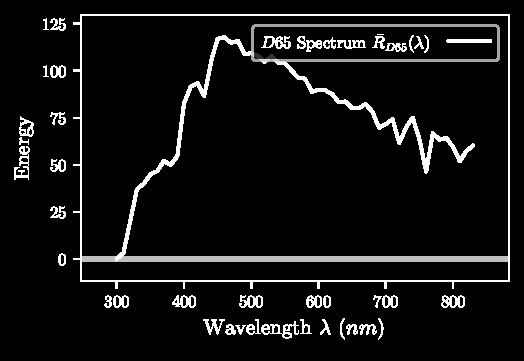
\includegraphics{../images/figure_06_d65_spectrum_inverted.pdf}
    \else
        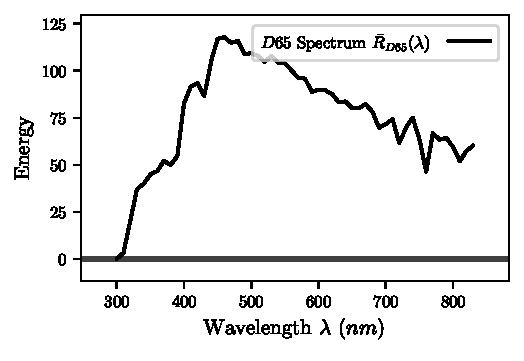
\includegraphics{../images/figure_06_d65_spectrum.pdf}
    \fi
    \captionof{figure}{CIE standard illuminant $D65$ energy spectrum.  IMAGE LINK, CODE LINK}\label{fig:d65_spectrum}
\end{halffigure}

\begin{figure*} % Figure 7
    \ifinvert
        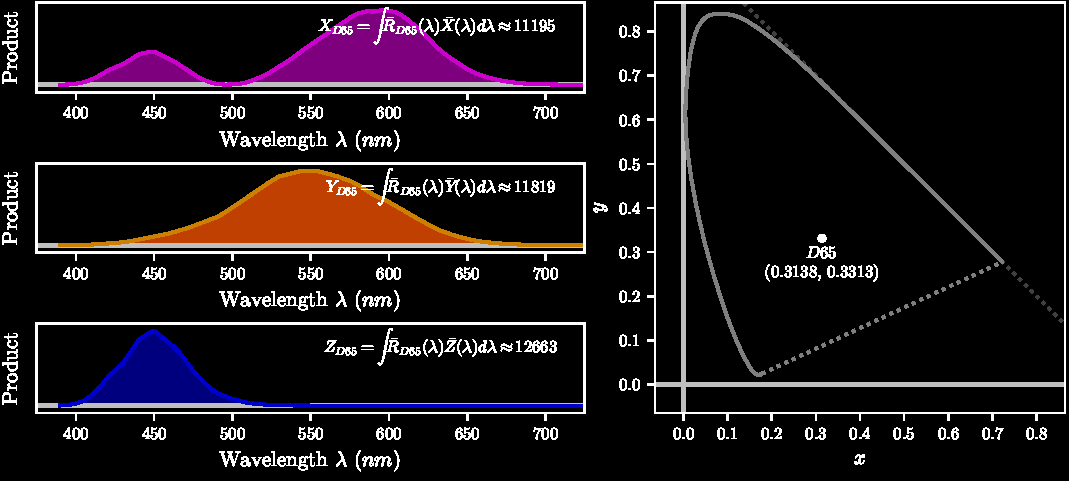
\includegraphics{../images/figure_07_estimating_d65_chromaticity_inverted.pdf}
    \else
        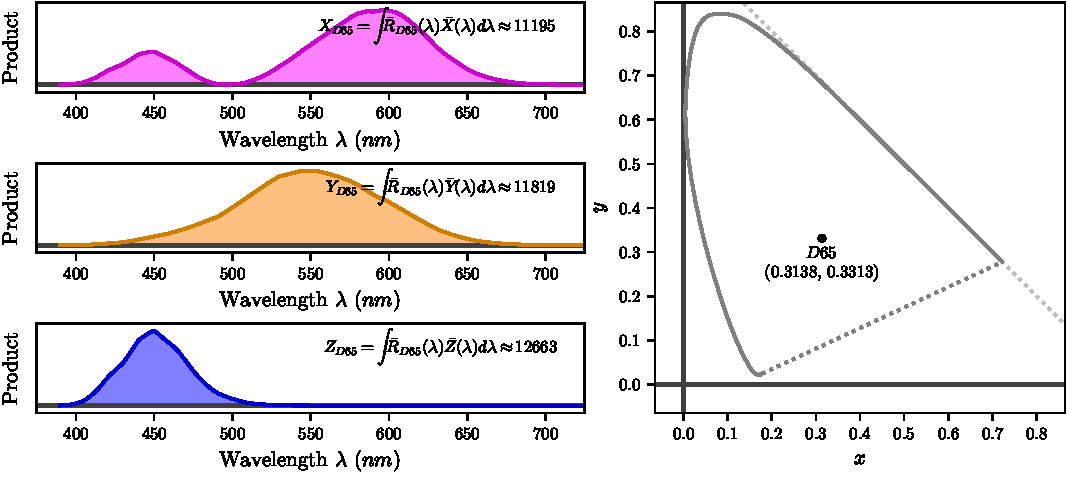
\includegraphics{../images/figure_07_estimating_d65_chromaticity.pdf}
    \fi
    \caption{Illustration of the estimation of chromaticity from a spectrum.  The three left panels show the products of the three color matching functions with the $D65$ spectrum.  The area shaded under each resulting curve is annotated within each panel by applying Equation \ref{eq:tristimulus_from_spectrum}.  The right panel shows the resulting chromaticity coordinate $(x,y)$ for the CIE 170-2 10$^\circ$ space (slightly different from the typically used CIE 1931).  IMAGE LINK, CODE LINK}\label{fig:estimating_d65_chromaticity}
\end{figure*}

Figure \ref{fig:d65_spectrum} shows the spectrum for the CIE standard illuminant $D65$ for average midday illumination (clear skies in Western / Northern Europe) (\cite{judd1964spectral}).  Such spectra will here be represented by $\bar{R}(\lambda)$ generally, and for this specific spectrum $\bar{R}_{D65}(\lambda)$.

The tristimulus values are found by multiplying each color matching function by the spectrum of interest and integrating to find the area under the resulting curves:

\begin{equation}\label{eq:tristimulus_from_spectrum} % Equation 15
    \begin{aligned}
        X&=\int\bar{R}(\lambda)\bar{X}(\lambda)d\lambda\\
        Y&=\int\bar{R}(\lambda)\bar{Y}(\lambda)d\lambda\\
        Z&=\int\bar{R}(\lambda)\bar{Z}(\lambda)d\lambda
    \end{aligned}
\end{equation}

To convert to chromaticity coordinates:

\begin{equation}\label{eq:chromaticity_from_tristimulus} % Equation 16
    \begin{aligned}
        x&=\frac{X}{X+Y+Z}\\
        y&=\frac{Y}{X+Y+Z}\\
        z&=\frac{Z}{X+Y+Z}\\
        \therefore 1&=x+y+z
    \end{aligned}
\end{equation}

Given the shared denominator for all three coordinates, any one can be found given the other two, so $z$ is typically left out of the discussion.  Figure \ref{fig:estimating_d65_chromaticity} illustrates the process of determining chromaticity from the $D65$ spectrum.

\subsubsection{Spectrum Locus} % 2.3.4

Chromaticity diagrams typically depict the “spectrum locus” which is the inverted “U” shape that represents the boundary within which all physically real colors - the chromaticities resulting from all possible spectra - lie.  This is based on the notion that the most extreme chromaticities arise from the narrowest possible single-wavelength spectra (i.e. pure, monochromatic lights) and all other possible spectra must be some mix of wavelengths and therefore fall within the line of monochromatic spectra - the spectrum locus.  The chromaticity coordinates of the spectrum locus are given by:

\begin{equation} % Equation 17
    \begin{aligned}
        \bar{x}(\lambda)=\frac{\bar{X}(\lambda)}{\bar{X}(\lambda)+\bar{Y}(\lambda)+\bar{Z}(\lambda)}\\
        \bar{y}(\lambda)=\frac{\bar{Y}(\lambda)}{\bar{X}(\lambda)+\bar{Y}(\lambda)+\bar{Z}(\lambda)}
    \end{aligned}
\end{equation}

using the color matching functions themselves ($\bar{X}(\lambda)$, $\bar{Y}(\lambda)$, and $\bar{Z}(\lambda)$).  The curved path with ends joined at the bottom by a dotted line depicted in Figure \ref{fig:estimating_d65_chromaticity} is the spectrum locus curve derived from the color matching functions (in Figure \ref{fig:color_matching_functions}) of the CIE 170-2 10$^\circ$ standard.

The differences among the CIE standards are slight, owing to updates and corrections over time arising from new experimental data or refinements of the underlying theory.  The difference between 10$^\circ$ and 2$^\circ$ standards arises from the difference in stimulus size, but this difference is usually only important under specific circumstances likely only to arise in psychophysical experiments themselves.  Figure \ref{fig:chromaticity_spaces} shows the spectrum loci and the chromaticity of $D65$ for a selection of CIE standards.  The CIE 170-2 standard (arguably the "modern" standard) has color matching functions for both 2$^\circ$ and 10$^\circ$ stimuli.  The CIE 1964 standard, based on a 10$^\circ$ stimulus, will come up later in the discussion of correlated color temperature (with a further conversion into a different chromaticity coordinate system).  The CIE 1931 standard - the original standard - using a 2$^\circ$ stimulus is still the most commonly cited standard and the one in which the sRGB system is defined.

\begin{halffigure} % Figure 8
    \ifinvert
        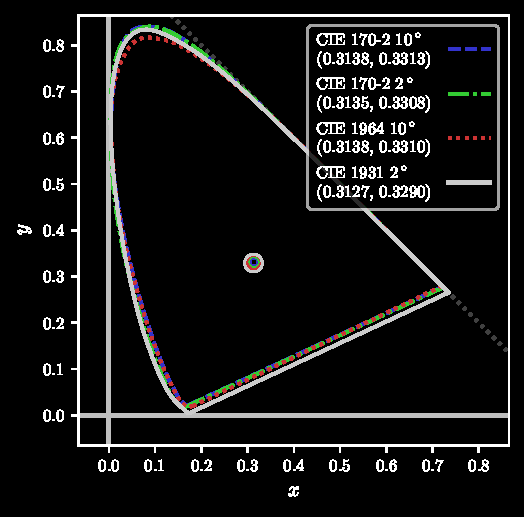
\includegraphics{../images/figure_08_chromaticity_spaces_inverted.pdf}
    \else
        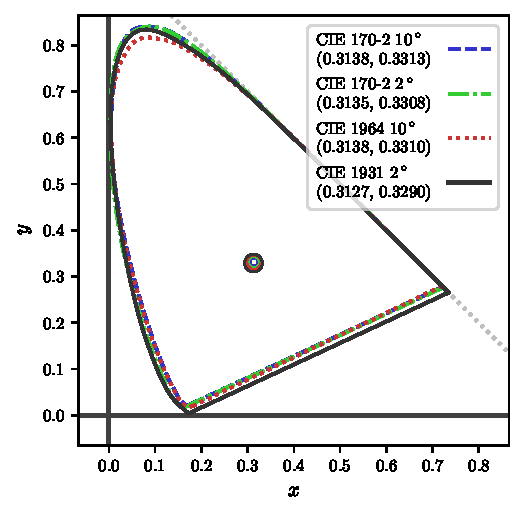
\includegraphics{../images/figure_08_chromaticity_spaces.pdf}
    \fi
    \captionof{figure}{Spectrum loci and $D65$ chromaticities for the CIE 170-2 10$^\circ$ and 2$^\circ$, 1964 10$^\circ$, and 1931 2$^\circ$ standards.  The chromaticity coordinates for $D65$ are given in the legend.  IMAGE LINK, CODE LINK}\label{fig:chromaticity_spaces}
\end{halffigure}

\subsubsection{Links} % 2.3.5

\begin{itemize}
    \item Article Full Text
    \begin{itemize}
        \item \cite{sharpe2011luminous} - \href{http://www.cvrl.org/people/Stockman/pubs/2011\%20Vstar\%20correction\%20SSJJ.pdf}{article page}
    \end{itemize}
    \item Colour \& Vision Research Laboratory
    \begin{itemize}
        \item \href{http://www.cvrl.org/ciexyzpr.htm}{Color Matching Functions (from CIE 2006 LMS)}
        \item \href{http://www.cvrl.org/database/text/cienewxyz/cie2012xyz10.htm}{10$^\circ$ Color Matching Functions Information}
        \item \href{http://www.cvrl.org/cie.htm}{CIE 1931 \& CIE 1964 Color Matching Functions}
    \end{itemize}
    \item Figure Images
    \begin{itemize}
        \item FIGURE 4 LIGHT AND DARK SVG
        \item FIGURE 5 LIGHT AND DARK SVG
        \item FIGURE 6 LIGHT AND DARK SVG
        \item FIGURE 7 LIGHT AND DARK SVG
        \item FIGURE 8 LIGHT AND DARK SVG
    \end{itemize}
    \item GitHub Scripts
    \begin{itemize}
        \item DATA INGESTION OF COLOR MATCHING FUNCTIONS AND CONVERSION TO SPECTRUM LOCI
        \item FIGURE GENERATION FOR ALL FIGURES (4-8)
    \end{itemize}
\end{itemize}

\end{multicols}

% ================ SECTION 3 ================

\begin{figure*} % Figure 9
    \ifinvert
        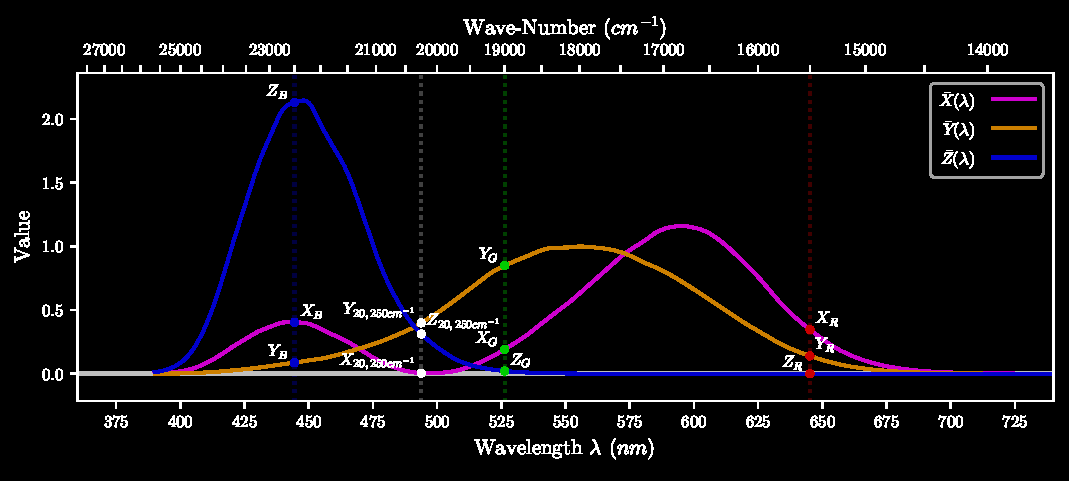
\includegraphics{../images/figure_09_color_matching_experiment_tristimulus_inverted.pdf}
    \else
        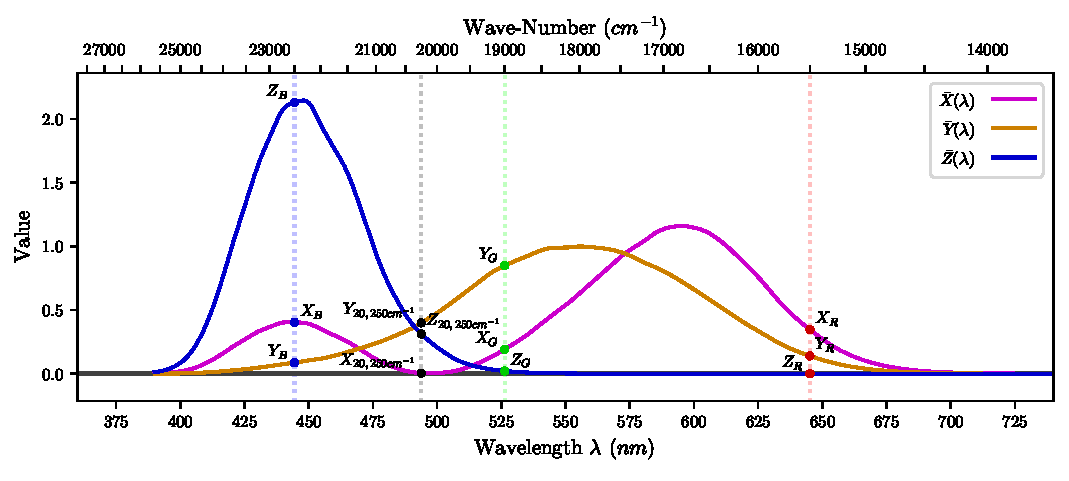
\includegraphics{../images/figure_09_color_matching_experiment_tristimulus.pdf}
    \fi
    \caption{CIE 170-2 10$^\circ$ color matching functions with the tristimulus values of the experiment primaries and the $20,250cm^{-1}$ test light annotated along the curves.  IMAGE LINK, CODE LINK}\label{fig:color_matching_experiment_tristimulus}
\end{figure*}

\section{Color Mixing} \label{sec:color_mixing}

\begin{multicols}{2}

To determine the chromaticity of a mix of two or more light sources we simply add up their tristimulus values ($X$, $Y$, and $Z$) and then apply Equation \ref{eq:chromaticity_from_tristimulus}.  This is demonstrated below first with the color matching experiment mean settings used to match the experiment primaries on the match side with the test light (and sometimes an experimental primary) on the test side.  Next are two demonstrations using the tristimulus values of color displays.

\subsection{Color Mixing in the Matching Experiment} % 3.1

The matching of mixed lights in the color matching experiment is easiest to arrange in a chromaticity diagram for the range of test colors between the green and blue primaries - where the green and blue settings are well above zero and contributing to the match side, and the red setting is well below zero and contributing to the test side - but the math is the same for any test light used in the experiment.  For this demonstration the test light with a wave-number of $20,250cm^{-1}$ is used, where the observers' averaged red, green, and blue settings are $\bar{R}(20,250cm^{-1})=-0.444$, $\bar{G}(20,250cm^{-1})=0.531$, and $\bar{B}(20,250cm^{-1})=0.144$, respectively.  The green and blue settings are positive and their tristimulus values are added together for the match side; the red setting is negative and its tristimulus values will be added to the test light's tristimulus values on the test side:

\begin{equation}\label{eq:match_tristimulus} % Equation 18
    \begin{aligned}
        \bar{G}(20,250cm^{-1})X_G+\bar{B}(20,250cm^{-1})X_B&=X_{match}\\
        \bar{G}(20,250cm^{-1})Y_G+\bar{B}(20,250cm^{-1})Y_B&=Y_{match}\\
        \bar{G}(20,250cm^{-1})Z_G+\bar{B}(20,250cm^{-1})Z_B&=Z_{match}
    \end{aligned}
\end{equation}

\begin{equation}\label{eq:test_tristimulus} % Equation 19
    \begin{aligned}
        X_{20,250cm^{-1}}-\bar{R}(20,250cm^{-1})X_R&=X_{test}\\
        Y_{20,250cm^{-1}}-\bar{R}(20,250cm^{-1})Y_R&=Y_{test}\\
        Z_{20,250cm^{-1}}-\bar{R}(20,250cm^{-1})Z_R&=Z_{test}
    \end{aligned}
\end{equation}

where $X_R$, $Y_R$, and $Z_R$ are the tristimulus values for the red primary, $X_G$, $Y_G$, and $Z_G$ are the tristimulus values for the green primary, $X_B$, $Y_B$, and $Z_B$ are the tristimulus values for the blue primary, and $X_{20,250cm^{-1}}$, $Y_{20,250cm^{-1}}$, and $Z_{20,250cm^{-1}}$ are the tristimulus values for the test light.  To get the tristimulus values for the three primaries and the test light we simply go to those wave-numbers/wavelengths on each of the color matching functions; we are treating these as ideal, monochromatic light sources and so we can forego the multiplication and integration steps implied by Equation \ref{eq:tristimulus_from_spectrum} and just use the values of $\bar{X}(\lambda)$, $\bar{Y}(\lambda)$, and $\bar{Z}(\lambda)$.  Figure \ref{fig:color_matching_experiment_tristimulus} annotates the tristimulus values for the primary lights and the selected test light.

Factoring the tristimulus values into Equations \ref{eq:match_tristimulus} and \ref{eq:test_tristimulus} we can solve for both sides of the experimental stimulus:

\begin{equation} % Equation 20
    \begin{aligned}
        (0.531)0.192+(0.144)0.405&=X_{match}=0.160\\
        (0.531)0.850+(0.144)0.087&=Y_{match}=0.464\\
        (0.531)0.022+(0.144)2.130&=Z_{match}=0.318
    \end{aligned}
\end{equation}

\begin{equation} % Equation 21
    \begin{aligned}
        0.005-(-0.444)0.347&=X_{test}=0.159\\
        0.400-(-0.444)0.140&=Y_{test}=0.462\\
        0.313-(-0.444)0.000&=Z_{test}=0.310
    \end{aligned}
\end{equation}

The tristimulus values on the match and test sides line up reasonably well, though not perfectly due to rounding at various steps (including the tabulated color matching functions).  Using the tristimulus values for the primaries and the selected test light we can get their chromaticities using Equation \ref{eq:chromaticity_from_tristimulus}: Red = $(0.713,0.287)$, Green = $(0.180,0.799)$, Blue = $(0.154,0.033)$ and for the $20,250cm^{-1}$ test light we get $(0.007,0.559)$.  The match and test chromaticities come to $(0.170,0.492)$ and $(0.171,0.496)$, respectively - again, reasonably similar.  Plotting all of these on a chromaticity diagram (see Figure \ref{fig:color_matching_experiment_mixing}) demonstrates that the mixing of two lights results in a chromaticity falling along a straight line between them, and in the case of the color matching experiment the resulting stimulus chromaticity is the point where the lines connecting the two lights contributing to either side of the stimulus intersect with one another.

\begin{halffigure} % Figure 10
    \ifinvert
        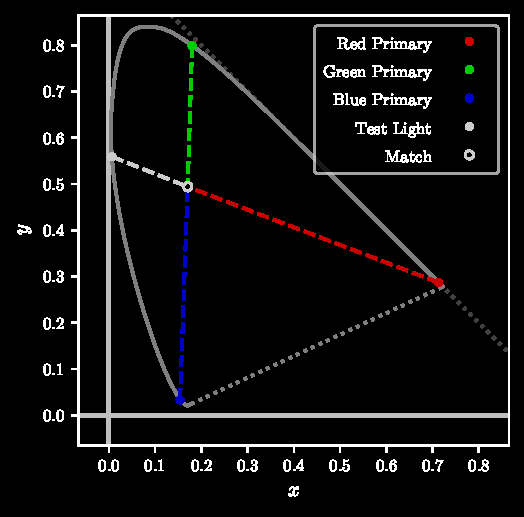
\includegraphics{../images/figure_10_color_matching_experiment_mixing_inverted.pdf}
    \else
        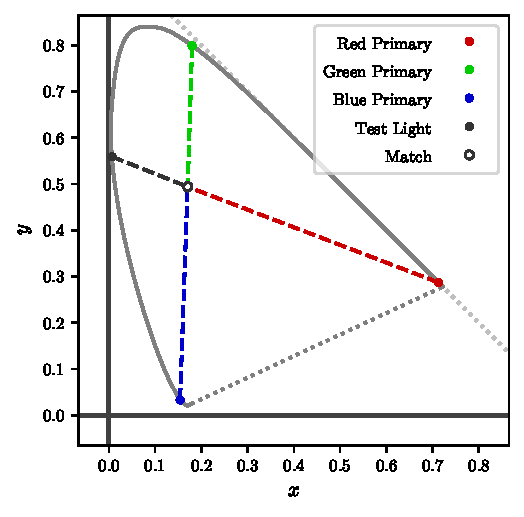
\includegraphics{../images/figure_10_color_matching_experiment_mixing.pdf}
    \fi
    \captionof{figure}{Chromaticities of the experimental primaries and the $20,250cm^{-1}$ test light.  The green and blue primaries on the match side of the stimulus, and the test light and red primary on the test side of the stimulus, are mixed in proportions to find the chromaticity where the lines joining each pair intersect.  IMAGE LINK, CODE LINK}\label{fig:color_matching_experiment_mixing}
\end{halffigure}

\subsection{Three-Primary Systems for Color Displays} % 3.2

For various practical reasons color displays typically do not use primary lights with anything near zero-width spectra.  Below, spectral measurements of an old cathode-ray-tube (CRT) monitor are used to define the range of colors that can be viewed on it.  Making certain simplifying assumptions, a linear transformation is constructed to allow any displayed color to be converted into chromaticity.

\subsubsection{Primary Chromaticities from Spectra} % 3.2.1

Figure \ref{fig:crt_monitor} shows the measured spectra of the red, green, and blue phosphors of a CRT monitor; note that above each is a curve showing the sum of all three spectra which corresponds to white.  Just as adding up tristimulus values (the integrated products of spectra and color matching functions) for the three primaries gives the tristimulus values for white, adding up the three spectra and estimating the tristimulus values once from that resulting spectrum should give the same result.

\begin{figure*} % Figure 11
    \ifinvert
        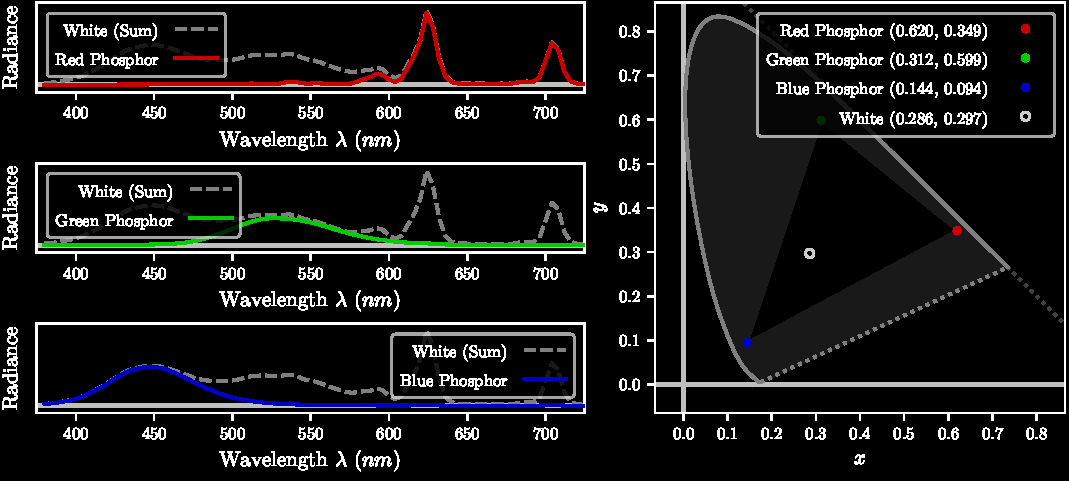
\includegraphics{../images/figure_11_crt_monitor_inverted.pdf}
    \else
        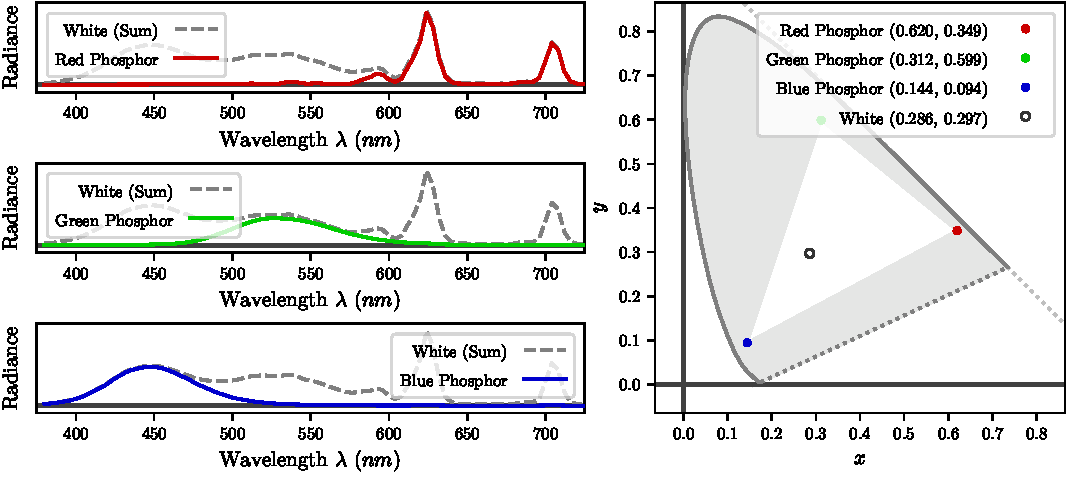
\includegraphics{../images/figure_11_crt_monitor.pdf}
    \fi
    \caption{Red, green, and blue phosphor spectra measured from a CRT monitor.  Above each spectral line is also shown the summed spectrum of white (dashed line).  The right panel plots the chromaticities (within the CIE 170-2 10$^\circ$ standard) of the three phosphors and white; the triangle formed by the three primaries is the monitor's color gamut.  All colors that can be shown by combining the three phosphors at various intensities fall within the color gamut triangle.  IMAGE LINK, CODE LINK}\label{fig:crt_monitor}
\end{figure*}

The chromaticity diagram in Figure \ref{fig:crt_monitor} plots the resulting chromaticities of the three CRT phosphors and the coordinate for white resulting from the addition of all three together at maximum intensity.  By changing the ratio of intensity of the three phosphors, any chromaticity within the triangle formed by the phosphor chromaticities can be realized.  This is the monitor's color gamut.

\subsubsection{Conversion between Display RGB and Chromaticity} % 3.2.2

If we assume that the shape of each phosphor spectrum remains the same as intensity increases and decreases, and that intensity increases and decreases in a linear fashion, we can express the tristimulus values resulting from any combination of red, green, and blue phosphor intensities ($R$, $G$, and $B$, respectively, each in the interval $[0,1]$) with the following linear combinations:

\begin{equation} % Equation 22
    \begin{aligned}
        X_RR+X_GG+X_BB&=X\\
        Y_RR+Y_GG+Y_BB&=Y\\
        Z_RR+Z_GG+Z_BB&=Z
    \end{aligned}
\end{equation}

or as the linear transform:

\begin{equation} % Equation 23
    \begin{bmatrix}
        X_R&X_G&X_B\\
        Y_R&Y_G&Y_B\\
        Z_R&Z_G&Z_B
    \end{bmatrix}\begin{bmatrix}
        R\\
        G\\
        B
    \end{bmatrix}=\begin{bmatrix}
        X\\
        Y\\
        Z
    \end{bmatrix}
\end{equation}

Filling in the tristimulus values for the CRT phosphors gives:

\begin{equation}\label{eq:crt_transformation} % Equation 24
    \begin{bmatrix}
        0.011376&0.009225&0.007038\\
        0.006395&0.017709&0.004606\\
        0.000573&0.002638&0.037099
    \end{bmatrix}\begin{bmatrix}
        R\\
        G\\
        B
    \end{bmatrix}=\begin{bmatrix}
        X\\
        Y\\
        Z
    \end{bmatrix}
\end{equation}

Once again, applying Equation \ref{eq:chromaticity_from_tristimulus} allows then for conversion into chromaticity coordinates.  In reality, the phosphor spectra do not perfectly maintain their shape with changes in intensity, nor does intensity change in a perfectly linear fashion, and so measuring and correcting for such deviations is important for experimental settings where precise chromaticity and luminance are desired.

\subsection{Links} % 3.3

\begin{itemize}
    \item CRT MONITOR SPECTRA
    \item Figure Images
    \begin{itemize}
        \item FIGURE 9 LIGHT AND DARK SVG
        \item FIGURE 10 LIGHT AND DARK SVG
        \item FIGURE 11 LIGHT AND DARK SVG
    \end{itemize}
    \item GitHub Scripts
    \begin{itemize}
        \item DATA INGESTION OF CRT PHOSPHOR SPECTRA
        \item FIGURE GENERATION FOR ALL FIGURES (9-11)
    \end{itemize}
\end{itemize}

\end{multicols}

% ================ SECTION 4 ================

\section{Chromaticity Diagram Coloration} \label{sec:chromaticity_coloration}

\begin{multicols}{2}

\begin{figure*} % Figure 12
    \ifinvert
        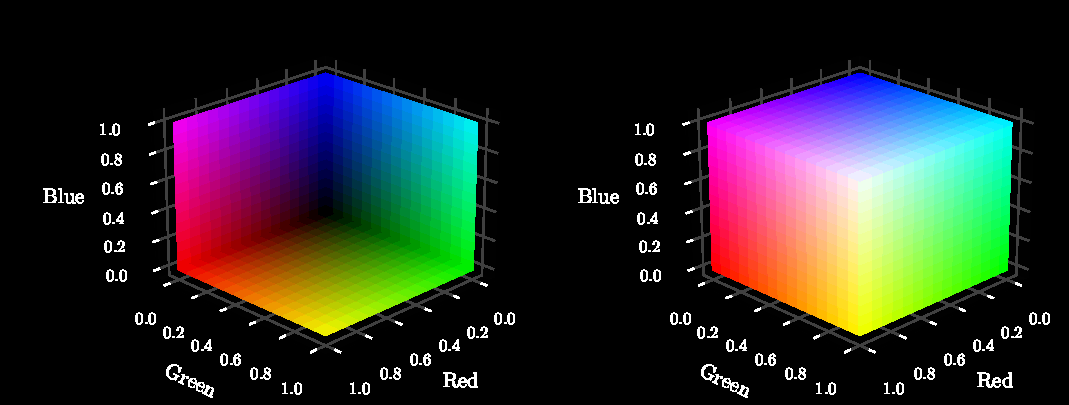
\includegraphics{../images/figure_12_3d_srgb_inverted.pdf}
    \else
        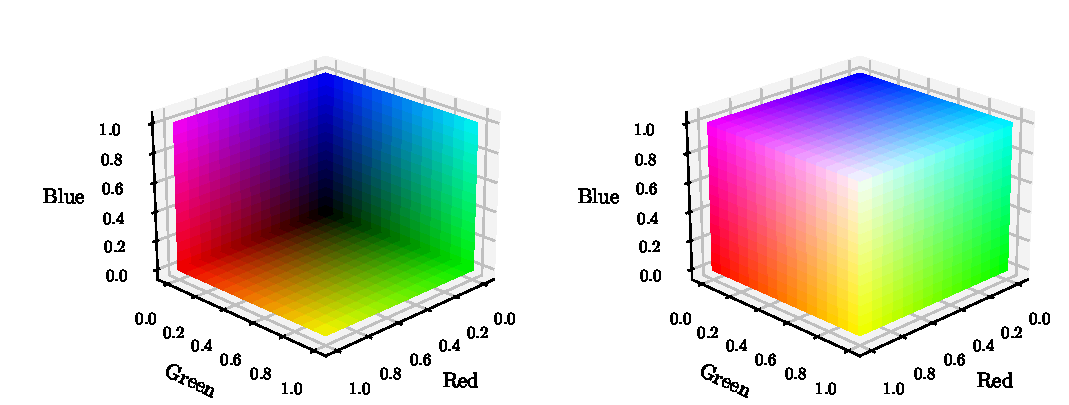
\includegraphics{../images/figure_12_3d_srgb.pdf}
    \fi
    \caption{Saturated surfaces of the sRGB color space cube.  In the left panel, all colors contain at least one 0.0 for red, green, and/or blue.  In the right panel, all colors contain at least one 1.0 for red, green, and/or blue.  IMAGE LINK, CODE LINK}\label{fig:3d_srgb}
\end{figure*}

\begin{figure*} % Figure 13
    \ifinvert
        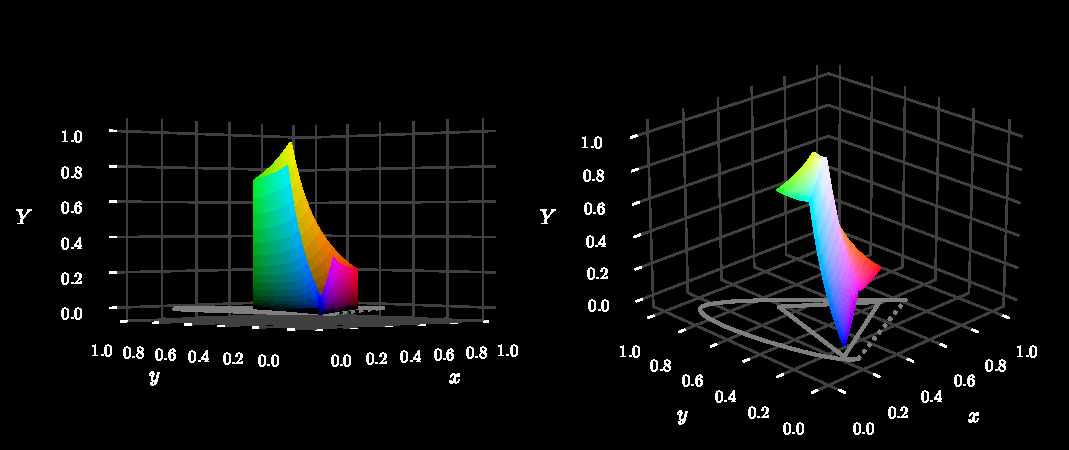
\includegraphics{../images/figure_13_3d_chromoluminance_inverted.pdf}
    \else
        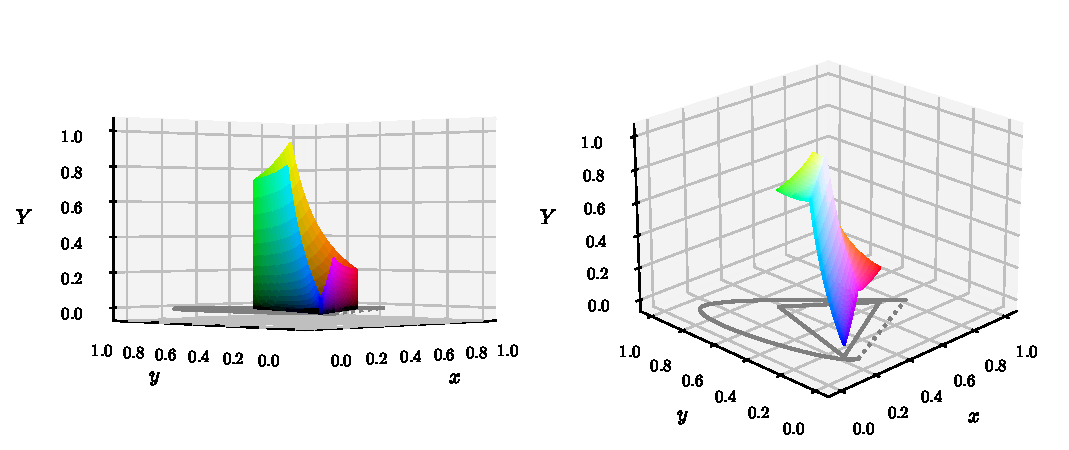
\includegraphics{../images/figure_13_3d_chromoluminance.pdf}
    \fi
    \caption{Saturated surfaces transformed into $(x,y,Y)$ chromoluminance space.  In the left panel, all colors contain at least one 0.0 for red, green, and/or blue (before transformation).  In the right panel, all colors contain at least one 1.0 for red, green, and/or blue (before transformation).  IMAGE LINK, CODE LINK}\label{fig:3d_chromoluminance}
\end{figure*}

There is no way to create a figure of the CIE $(x,y)$ chromaticity diagram where the interior of the spectrum locus is filled with accurate colors short of a complicated optical setup, and then it could only be viewed correctly in person - any pictures taken of the result would become false copies due to the limitations of the camera and the display on which the image is viewed.  Therefore, because compromises need to be made, we are free to choose how exactly we fill the space with color and there can’t be an objectively correct way to do so.  The area within the display gamut triangle is a bit more straightforward, so we’ll start there, and then expand the colors to fill the rest of the spectrum locus area.

\subsection{sRGB} % 4.1

In the previous section we used the CIE 170-2 10$^\circ$ color matching functions, and therefore plotted chromaticity in that space.  The sRGB display standard is defined with CIE 1931 2$^\circ$ tristimulus values, and so from this point on in the document the CIE 1931 2$^\circ$ standard will be used (this ultimately has only a slight effect on the coordinates plotted as is evident in Figure \ref{fig:chromaticity_spaces}).  The sRGB tristimulus values are given in the following linear transformation (similar in function to Equation \ref{eq:crt_transformation}) (\href{https://en.wikipedia.org/wiki/SRGB}{source}):

\begin{equation}\label{eq:srgb_transformation} % Equation 25
    \begin{bmatrix}
        0.4124&0.3576&0.1805\\
        0.2126&0.7152&0.0722\\
        0.0193&0.1192&0.9505
    \end{bmatrix}\begin{bmatrix}
        R\\
        G\\
        B
    \end{bmatrix}=\begin{bmatrix}
        X\\
        Y\\
        Z
    \end{bmatrix}
\end{equation}

Note that the sum of the second row, the $Y$ values for red, green, and blue, is equal to 1.0.  The sRGB system is set up so that the maximum "luminance" value is 1.0 for white when red, green, and blue are at maximum (1.0) and the tristimulus values also result in the chromaticity of white being that of the $D65$ standard illuminant $(0.3127,0.3290)$.

There is an additional step that will be treated as optional here depending on the desired outcome, that of gamma correction.  This is meant to linearize values before they are converted into tristimulus values.  Before applying Equation \ref{eq:srgb_transformation} above, the red, green, and blue values are adjusted with:

\begin{equation}\label{eq:gamma_correction} % Equation 26
    C_{linear}=\left\{\begin{array}{ll}
        \frac{C_{srgb}}{12.92}&C_{srgb}\leq0.04045\\
        \left(\frac{C_{srgb}+0.055}{1.055}\right)^{2.4}&C_{srgb}>0.04045
    \end{array}\right.
\end{equation}

Applying this correction will provide a more accurate depiction of luminance in 3D, but will create an (arguably) unsightly discontinuity in 2D.

\subsection{Three-Dimensional Color Spaces} % 4.2

The sRGB space, or any red-green-blue space, can be visualized as a cube in three-dimensions with each dimension corresponding to a primary color.  Figure \ref{fig:3d_srgb} shows the six exterior surfaces of the cube, here called saturation surfaces as at least one of red, green, or blue is equal to 0.0 or 1.0.  All possibly display colors are contained within the cube.

To visualize chromoluminance (chromaticity and luminance), the colors in Figure \ref{fig:3d_srgb} are passed through gamma-correction (Equation \ref{eq:gamma_correction}) and transformed to tristimulus values using Equation \ref{eq:srgb_transformation}.  We hang on to $Y$ to represent luminance, and use Equation \ref{eq:chromaticity_from_tristimulus} to get $(x,y)$ chromaticity coordinates.  The resulting transformation of the saturation surfaces in chromoluminance space is presented in Figure \ref{fig:3d_chromoluminance}.

The shape of the sRGB color gamut in three-dimensional chromoluminance space is far from a regular cube.  The six sides of the original cube in Figure \ref{fig:3d_srgb} maintain the same shared edges with one another, and the vertices still come to points at red, yellow, green, cyan, blue, pink, black, and white, but the shape of each side undergoes all manner of transformations.  One important feature to note is that the luminances $Y$ of the different primary colors (red, green, and blue) are different.  The right panel of Figure \ref{fig:3d_chromoluminance} shows the color gamut narrowing as one increases luminance which means the available range of chromaticities is constricting; this also happens at the bottom as one approaches black, but over a much shorter luminance range, and one must arbitrarily assign a chromaticity to black itself to deal with divide-by-zero issues with Equation \ref{eq:chromaticity_from_tristimulus} when $X+Y+Z=0$.

\subsection{Two-Dimensional, Top-Down Chromaticity} % 4.3

To begin adding color to our chromaticity diagrams, we can rotate the right panel in Figure \ref{fig:3d_chromoluminance} to give a top-down view (see Figure \ref{fig:chromaticity_inside_gamut}), which shows an attractive range of highly saturated colors.  Remember that we are looking down at the top of an irregularly shaped volume with a peak at white - these colors do not represent a flat surface, even though we are rendering them in two dimensions.

\begin{halffigure} % Figure 14
    \ifinvert
        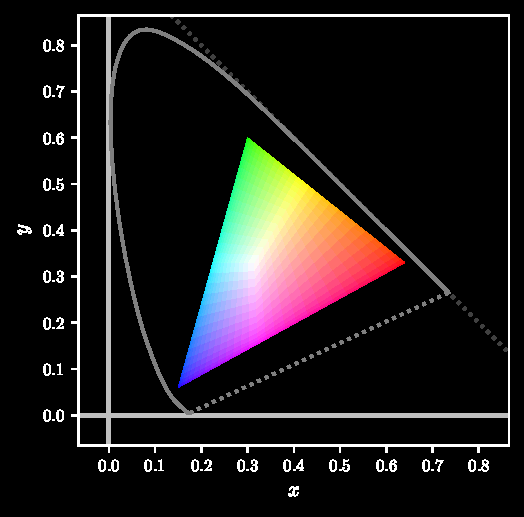
\includegraphics{../images/figure_14_chromaticity_inside_gamut_inverted.pdf}
    \else
        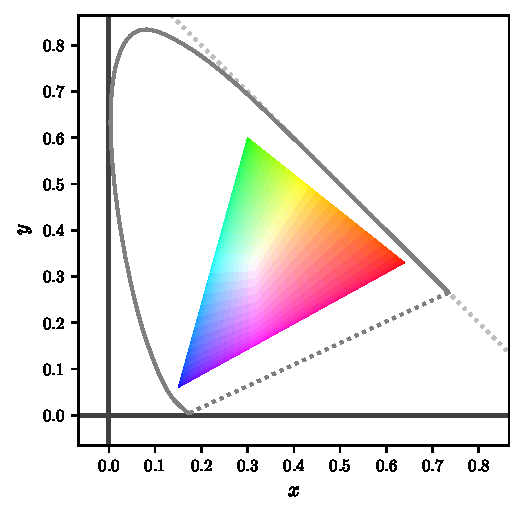
\includegraphics{../images/figure_14_chromaticity_inside_gamut.pdf}
    \fi
    \captionof{figure}{Top-down view of the sRGB color gamut transformed into chromoluminance space (here two-dimensional chromaticity) which effectively fills the chromaticity color gamut with color.  IMAGE LINK, CODE LINK}\label{fig:chromaticity_inside_gamut}
\end{halffigure}

\subsubsection{Extending Color beyond the sRGB Color Gamut Triangle} % 4.3.1

Looking down at the sRGB color gamut, it appears that a given angle around white maintains constant hue (named color) while increasing in saturation (chromatic contrast) moving away from white in that direction.  This idea can be used to fill the area outside the triangle with color by simply finding the hue for a given angle around white and extending a wedge of constant, saturated color outward (see Figure \ref{fig:chromaticity_outside_gamut}).

\begin{figure*} % Figure 15
    \ifinvert
        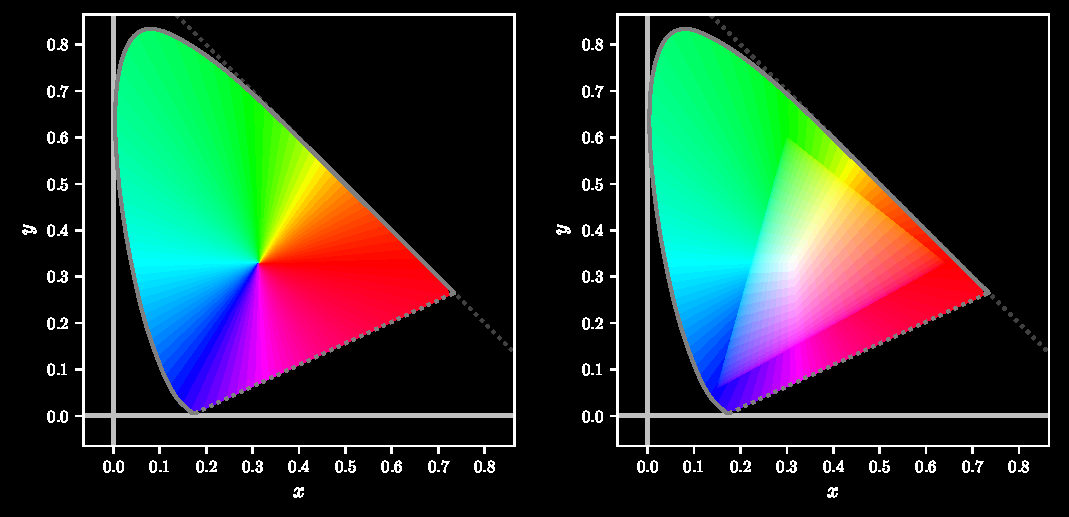
\includegraphics{../images/figure_15_chromaticity_outside_gamut_inverted.pdf}
    \else
        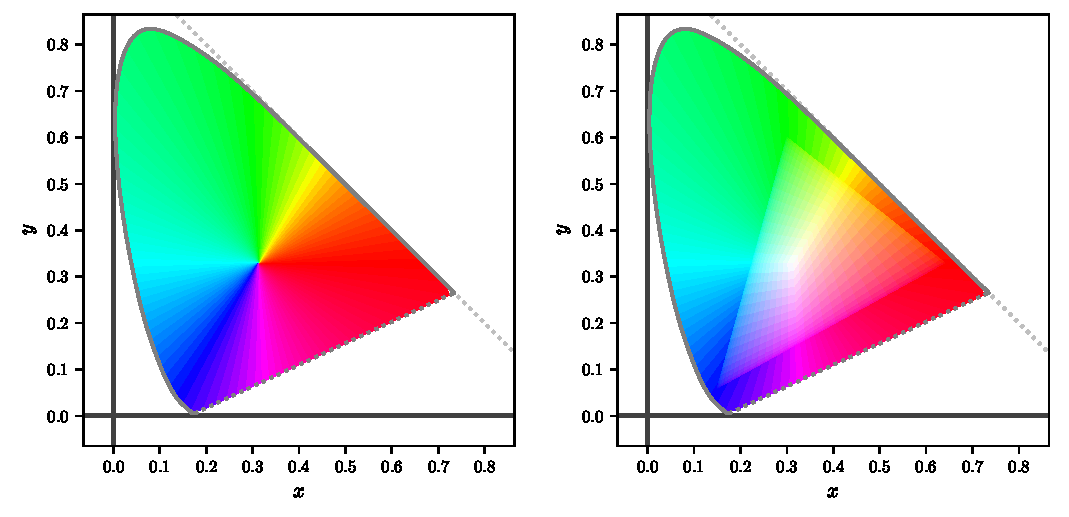
\includegraphics{../images/figure_15_chromaticity_outside_gamut.pdf}
    \fi
    \caption{Filling in colors outside of the color gamut triangle (but within the CIE 1931 2$^\circ$ spectrum locus).  The method applied does not vary in color saturation (see left panel where the central point is not white), but the top-down view of high-saturation surfaces can be placed on top (see right panel).  Note that the colors within the triangle in the right panel are less saturated than the colored region outside the triangle creating a discontinuity (i.e. the triangle edges are apparent).  IMAGE LINK, CODE LINK}\label{fig:chromaticity_outside_gamut}
\end{figure*}

\subsubsection{Effects of Gamma Correction} % 4.3.2

\begin{halffigure} % Figure 16
    \ifinvert
        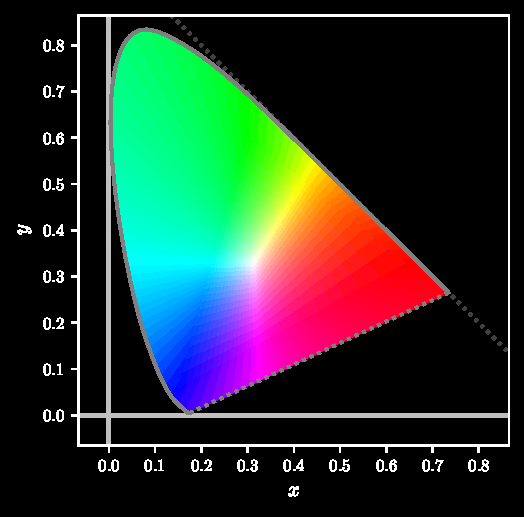
\includegraphics{../images/figure_16_chromaticity_without_gamma_correction_inverted.pdf}
    \else
        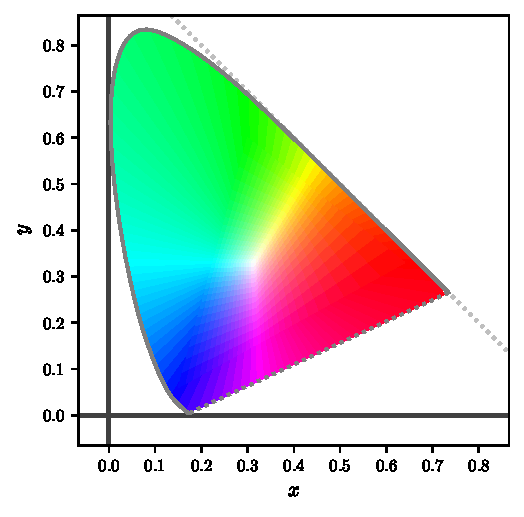
\includegraphics{../images/figure_16_chromaticity_without_gamma_correction.pdf}
    \fi
    \captionof{figure}{Color-filled chromaticity diagram with no gamma correction applied when coloring in the region inside the sRGB color gamut triangle.  Note that the edges of the color gamut triangle are no longer apparent.  IMAGE LINK, CODE LINK}\label{fig:chromaticity_without_gamma_correction}
\end{halffigure}

The discontinuity seen in Figure \ref{fig:chromaticity_outside_gamut} can be solved by \textit{not} applying gamma correction (see Figure \ref{fig:chromaticity_without_gamma_correction}) when filling in the colors inside the color gamut triangle (the method for coloring the rest of the diagram is not impacted by gamma correction either way).  This makes for an arguably more attractive diagram (and will be used for the remainder of this document), however Figure \ref{fig:gamma_correction_in_chromoluminance} demonstrates why applying gamma correction is the more technically correct approach (at least in three dimensions).  Note that when applying gamma correction (left panel of Figure \ref{fig:gamma_correction_in_chromoluminance}) the brightness of the colored pixels increases with increasing luminance $Y$, however without gamma correction (right panel) the apparent brightness is not consistent for a given luminance (see how the bright blue point of the blue primary is surrounded by darker pixels that are supposed to have the same luminance).  The edge tracing from one primary color to the next (red to yellow to green to cyan to blue to pink and back to red) is the same with or without gamma correction, so technically there is no discontinuity in the right panel of Figure \ref{fig:chromaticity_outside_gamut}, but you would have to zoom in closely to see a smooth gradient of saturation near the triangle edges.

\begin{figure*} % Figure 17
    \ifinvert
        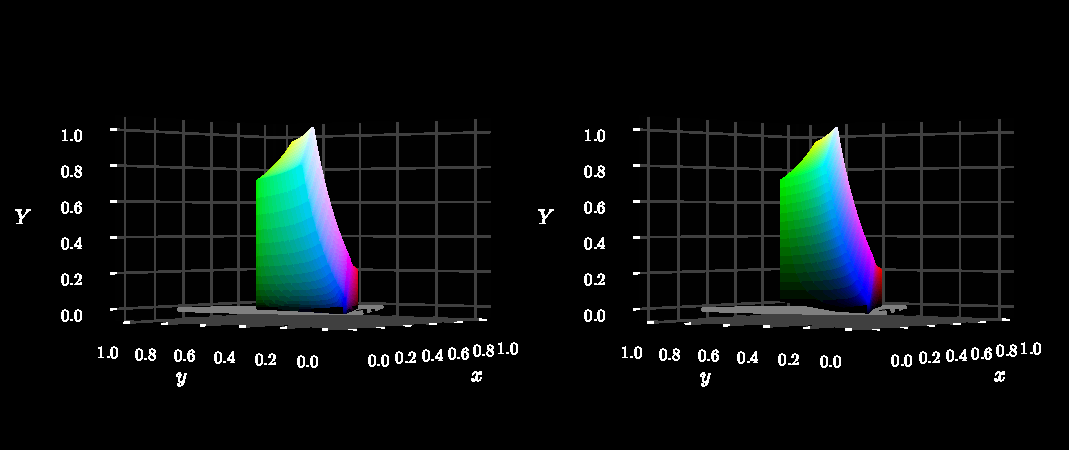
\includegraphics{../images/figure_17_gamma_correction_in_chromoluminance_inverted.pdf}
    \else
        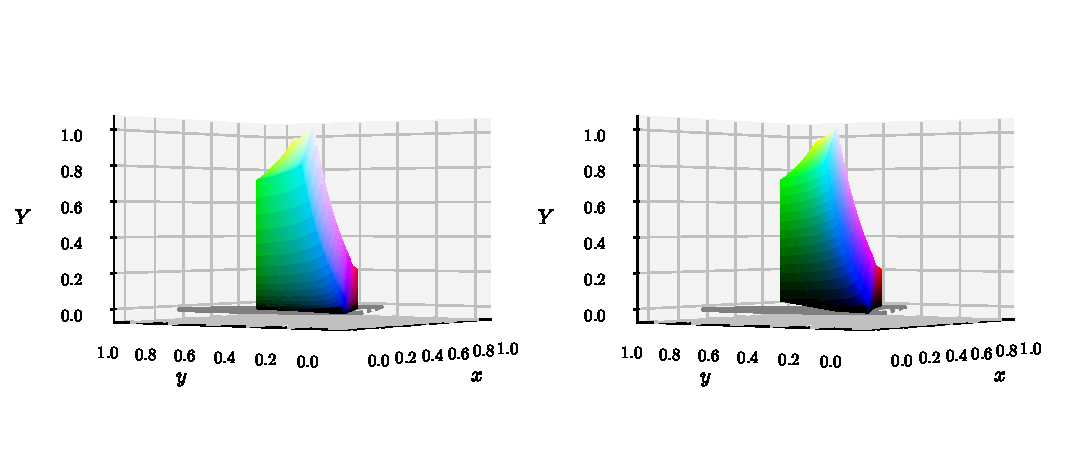
\includegraphics{../images/figure_17_gamma_correction_in_chromoluminance.pdf}
    \fi
    \caption{Saturated surfaces transformed into $(x,y,Y)$ chromoluminance space with (left panel) and without (right panel) gamma correction applied.  With gamma correction the apparent brightness of pixels increases with luminance $Y$ uniformly around the color gamut volume.  Without gamma correction the sides generally appear darker, yet the brightness is still high near the primary colors creating variation in apparent brightness around what should be a path of constant luminance.  IMAGE LINK, CODE LINK}\label{fig:gamma_correction_in_chromoluminance}
\end{figure*}

\subsection{The Visible Spectrum} % 4.4

Creating a band of colors that represents the visible spectrum, effectively finding red, green, and blue values as a function of wavelength, is a simple matter of taking our color-filled chromaticity diagram and grabbing the colors from along the spectrum locus curve.  Figure \ref{fig:visible_spectrum_locus} shows what this looks like based on how we've added color to the chromaticity diagram.  Along the spectrum locus (indeed everywhere outside of the color gamut triangle) all colors have at least one 0.0 and one 1.0 for red, green, and/or blue which results in saturated colors and relatively narrow transitions through cyan and yellow.

The wavelengths indicated for red, yellow, green, cyan, and blue are based here on the combination of the chromaticities of the sRGB primaries and their positions relative to the CIE 1931 2$^\circ$ spectrum locus.  Rotating a primary clockwise or counter-clockwise around the white point ($D65$ here) would increase or decrease the wavelength for that primary, respectively.  Additionally, the intermediate colors cyan, pink, and yellow are by our formulations necessarily 180$^\circ$ of hue angle away from red, green, and blue, respectively; therefore the wavelengths of red and cyan are not independent, nor are the wavelengths of blue and yellow.  Changing the white point would also impact the wavelengths of the named colors.  It is difficult to know what the proper wavelengths of the named colors are - any photograph of a spectrum of light that you view on a display is going to be influenced by both camera and display.  The wavelengths annotated in Figure \ref{fig:visible_spectrum_locus} are close enough to those found searching online, but if one wanted to customize their visible spectrum image a careful choosing of primary and white chromaticities could be undertaken.

Figure \ref{fig:visible_spectrum_functions} plots the red, green, and blue values as a function of wavelength based on the method described above.  Note that one of the three component colors is at minimum (0.0) and one is at maximum (1.0) throughout the whole range.  These saturated colors represent just one possible method that stays true to the hue angle for each wavelength.  Figure \ref{fig:visible_spectrum_functions} also shows a spectrum where the chromatic contrast and luminance profiles have been smoothed (in this case following Gaussian curves as functions of wavelength - not shown) resulting in red, green, and blue values that flow more continuously without sharp bends.

\begin{halffigure} % Figure 18
    \ifinvert
        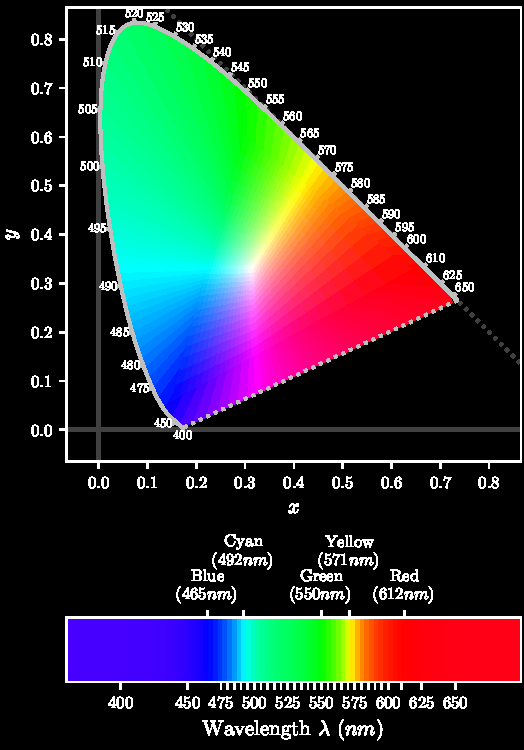
\includegraphics{../images/figure_18_visible_spectrum_locus_inverted.pdf}
    \else
        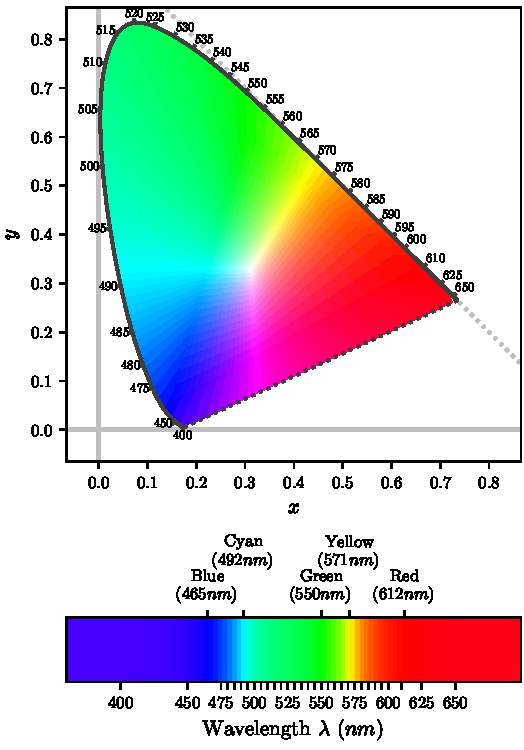
\includegraphics{../images/figure_18_visible_spectrum_locus.pdf}
    \fi
    \captionof{figure}{Color-filled chromaticity diagram with annotated wavelengths.  The vertical strip to the right shows the colors along the spectrum locus.  Named colors are annotated along with the closest whole wavelength match; these are the points where the saturated colors have only 0 or 1 in them (e.g. $(1,0,1)$ for yellow).  IMAGE LINK, CODE LINK}\label{fig:visible_spectrum_locus}
\end{halffigure}

\begin{figure*} % Figure 19
    \ifinvert
        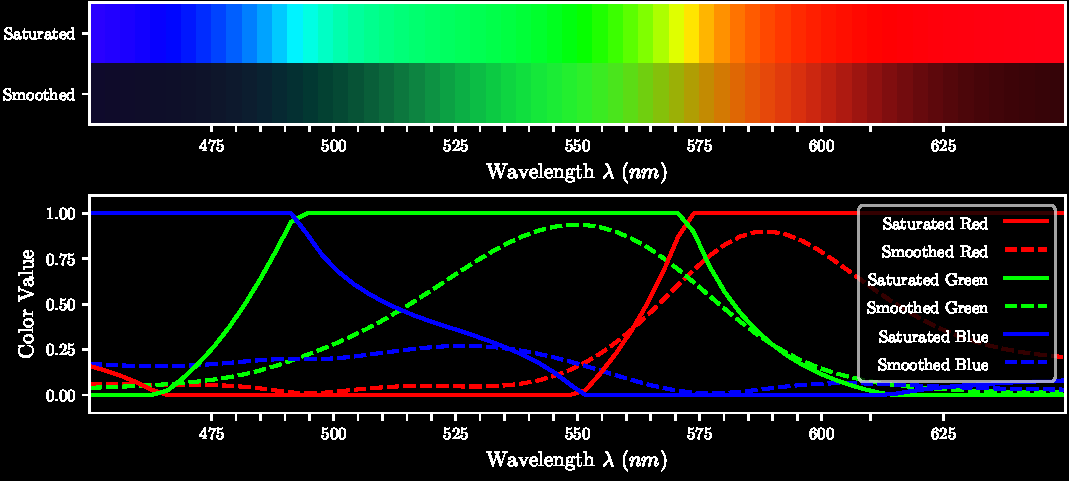
\includegraphics{../images/figure_19_visible_spectrum_functions_inverted.pdf}
    \else
        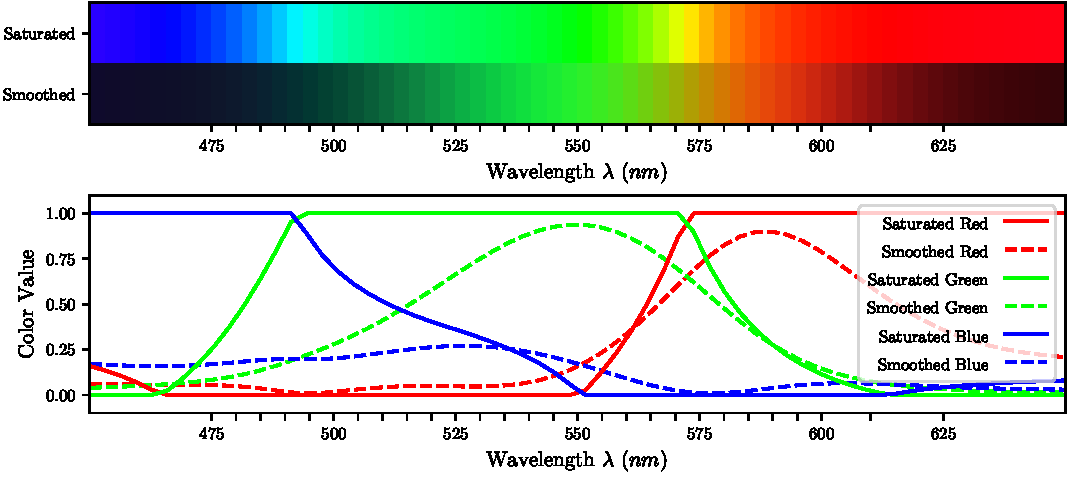
\includegraphics{../images/figure_19_visible_spectrum_functions.pdf}
    \fi
    \caption{Visible spectrum bands and the corresponding red, green, and blue values as functions of wavelengths.  The saturated spectrum is the same as that presented in Figure \ref{fig:visible_spectrum_locus} (with the more extreme wavelengths cropped out).  The smoothed spectrum was constructed with an arbitrary method that preserves the hue angle for each wavelength but otherwise smooths out the resulting functions for red, green, and blue (note that green and blue cross at the same cyan wavelength, and green and red cross at the same yellow wavelength, for both series).  IMAGE LINK, CODE LINK}\label{fig:visible_spectrum_functions}
\end{figure*}

\subsection{Links} % 4.5

\begin{itemize}
    \item \href{https://en.wikipedia.org/wiki/SRGB}{sRGB Wikipedia Article}
    \item Figure Images
    \begin{itemize}
        \item FIGURE 12 LIGHT AND DARK SVG
        \item FIGURE 13 LIGHT AND DARK SVG
        \item FIGURE 14 LIGHT AND DARK SVG
        \item FIGURE 15 LIGHT AND DARK SVG
        \item FIGURE 16 LIGHT AND DARK SVG
        \item FIGURE 17 LIGHT AND DARK SVG
        \item FIGURE 18 LIGHT AND DARK SVG
        \item FIGURE 19 LIGHT AND DARK SVG
    \end{itemize}
    \item GitHub Scripts
    \begin{itemize}
        \item FIGURE GENERATION FOR ALL FIGURES (12-19)
    \end{itemize}
\end{itemize}

\end{multicols}

% ================ SECTION 5 ================

\section{Color Temperature} \label{sec:color_temperature}

\begin{multicols}{2}

Many depictions of the CIE chromaticity diagram include annotations for the Planckian locus.  This line represents the change in chromaticity of blackbody radiation of increasing temperature, starting red and passing through white towards blue (for a fun diversion see “effective temperature” and “Hertzsprung-Russell diagram”).  Here we will introduce a transformed CIE chromaticity diagram using coordinates $(u,v)$ (\cite{cie_1960}) as the formulation of correlated color temperature is based on that space.

\subsection{Spectral Radiance of Blackbody Radiation} % 5.1

To determine the chromaticity associated with a particular temperature we will apply the CIE 1931 2$^\circ$ color matching functions to blackbody radiation spectra defined by Planck’s Law (\href{https://en.wikipedia.org/wiki/Planckian_locus}{source}):

\begin{equation} % Equation 27
    \begin{aligned}
        M(\lambda,T)&=\frac{c_1}{\lambda^5}\frac{1}{e^{\frac{c_2}{\lambda T}}-1}\\
        c_1&=2\pi hc^2\\
        c_2&=\frac{hc}{k}
    \end{aligned}
\end{equation}

where $M$ is the spectral radiance as a function of wavelength $\lambda$ and temperature $T$.  $h$, $c$, and $k$ are Planck's constant, the speed of light, and Boltzmann's constant, respectively.  Just as we did with the CRT monitor spectra, we'll integrate the product of each color matching function with the blackbody radiation spectrum for a given temperature:

\begin{equation} % Equation 28
    \begin{aligned}
        X(T)&=\int M(\lambda,T)\bar{X}(\lambda)d\lambda\\
        Y(T)&=\int M(\lambda,T)\bar{Y}(\lambda)d\lambda\\
        Z(T)&=\int M(\lambda,T)\bar{Z}(\lambda)d\lambda
    \end{aligned}
\end{equation}

and then apply Equation \ref{eq:chromaticity_from_tristimulus} to get $(x,y)$ chromaticity.  Figure \ref{fig:blackbody_spectra} shows a selection of blackbody spectra and their corresponding chromaticity coordinates annotated along the Planckian locus.  While low temperatures fall off the chromaticity diagram beyond red (a thing ought to be at least "red hot" to be visible) the highest temperatures do not venture very far into blue territory, approaching asymptotically towards $\approx(0.2400, 0.2340)$.

\begin{figure*} % Figure 20
    \ifinvert
        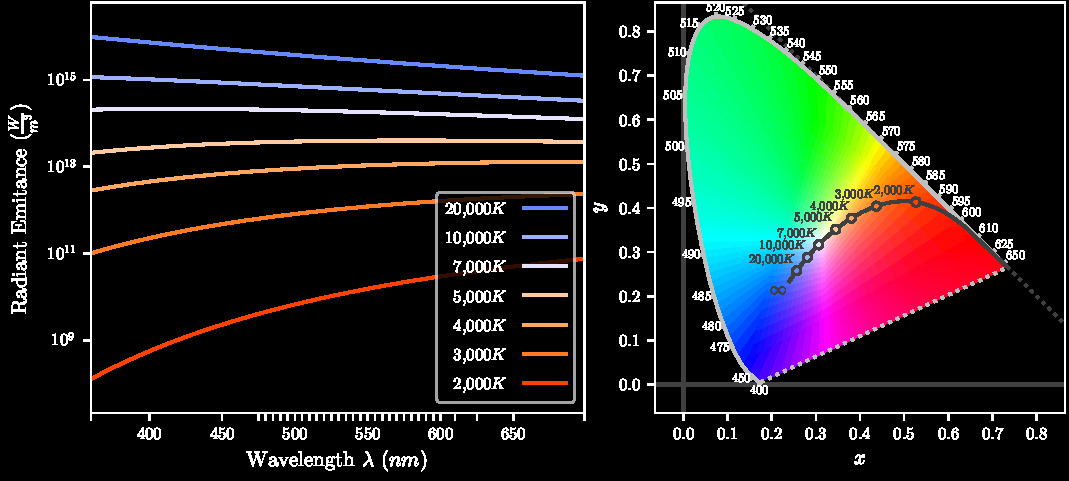
\includegraphics{../images/figure_20_blackbody_spectra_inverted.pdf}
    \else
        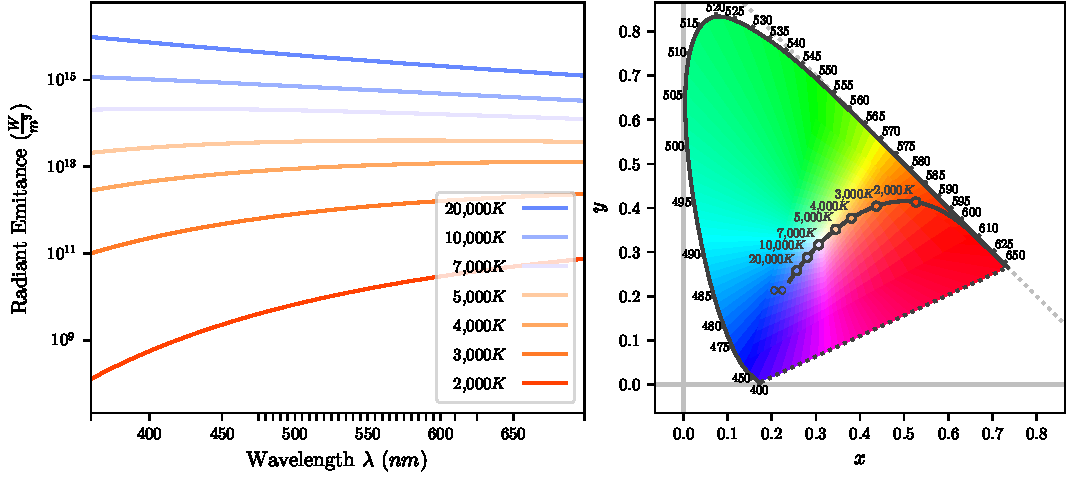
\includegraphics{../images/figure_20_blackbody_spectra.pdf}
    \fi
    \caption{Blackbody spectra for selected temperatures and their chromaticities plotted along the Planckian locus in CIE 1931 2$^\circ$ $(x,y)$ chromaticity space.  Note that the Planckian locus is not actually drawn out to infinity - it ends at $10^{10}K$ here - but chromaticity changes become infinitesimal as temperatures become infinite.  IMAGE LINK, CODE LINK}\label{fig:blackbody_spectra}
\end{figure*}

\subsection{Correlated Color Temperature} % 5.2

The above formulation allows us to determine chromaticity from temperature.  In order to derive temperature from color we will invoke geometry within the CIE 1960 $(u,v)$ chromaticity diagram.  There are various approximating equations to estimate color temperature, but the original method of determining correlated color temperature is geometric (\cite{kelly1963lines}).

\subsubsection{Conversion between $(x,y)$ and $(u,v)$ Chromaticity Coordinates} % 5.2.1

The following conversions were offered by MacAdam (\cite{macadam1937projective}) to convert to/from the CIE 1960 "uniform color space" (work began in the 30s, but the standard apparently took a while to adopt):

\begin{equation} % Equation 29
    \begin{aligned}
        u&=\frac{4x}{12y-2x+3}\\
        v&=\frac{6y}{12y-2x+3}\\
        x&=\frac{3u}{2u-8v+4}\\
        y&=\frac{2v}{2u-8v+4}
    \end{aligned}
\end{equation}

Various attempts to make a uniform color space aim to make unit step changes in any direction, from any point in the chromaticity diagram, of perceptually similar magnitude.  This is an interesting topic for another time, but it is part of the reason why new color spaces continue to appear over time.  Figure \ref{fig:two_chromaticity_spaces} shows both chromaticity spaces side-by-side.

\begin{figure*} % Figure 21
    \ifinvert
        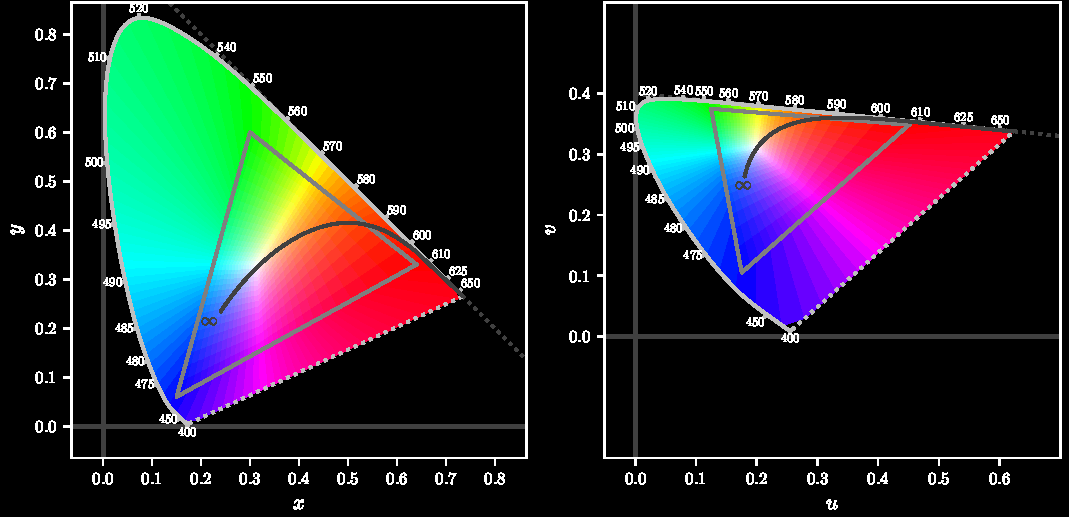
\includegraphics{../images/figure_21_two_chromaticity_spaces_inverted.pdf}
    \else
        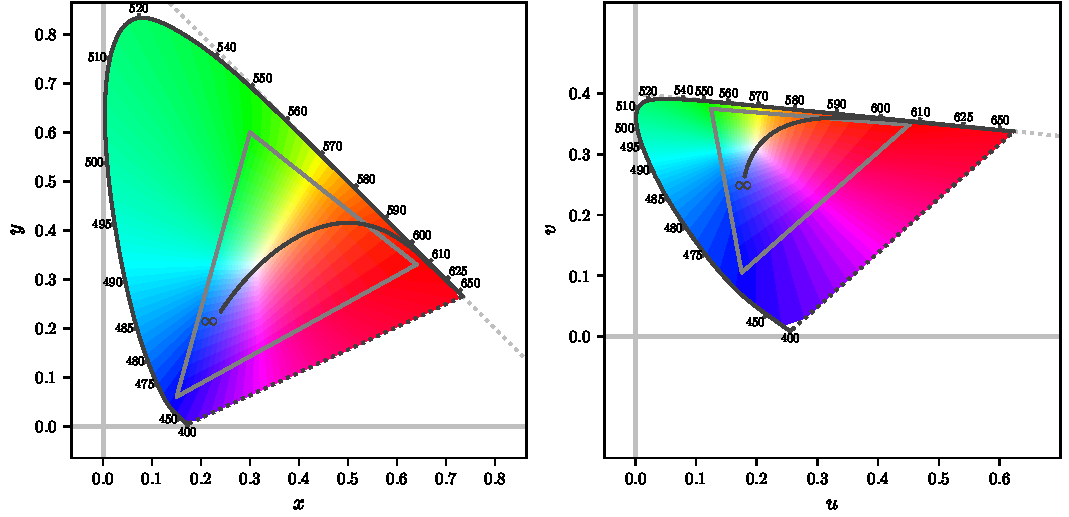
\includegraphics{../images/figure_21_two_chromaticity_spaces.pdf}
    \fi
    \caption{CIE 1931 $(x,y)$ (left) and CIE 1960 $(u,v)$ (right) chromaticity diagrams.  The sRGB color gamut triangle is present in both diagrams along with the Planckian locus.  IMAGE LINK, CODE LINK}\label{fig:two_chromaticity_spaces}
\end{figure*}

\subsubsection{Isotherm Lines} % 5.2.2

Any chromaticity that is within a distance of $0.05$ from the Planckian locus in the $(u,v)$ chromaticity diagram has a correlated color temperature equal to the temperature on the closest part of the Planckian locus.  This can be visualized by extending lines perpendicular from the Planckian locus out to that distance as shown in Figure \ref{fig:isotherm_lines_zoom}.  A selection of standard illuminants and their correlated color temperatures are plotted: illuminant $A$ represents a traditional incandescent / tungsten filament bulb, $D65$ is the clear day sky used as white in the sRGB standard, $E$ represents an equal-energy (i.e. horizontal) light spectrum and $F3$ (there are many $F$ illuminants) represents a white fluorescent bulb (\href{https://en.wikipedia.org/wiki/Standard_illuminant}{source}).

\begin{figure*} % Figure 22
    \ifinvert
        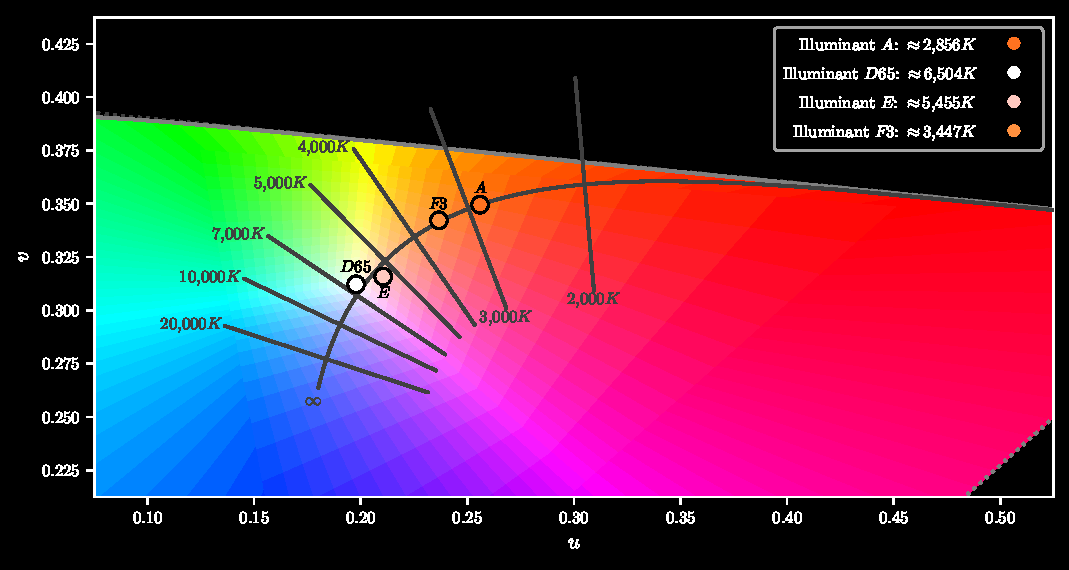
\includegraphics{../images/figure_22_isotherm_lines_zoom_inverted.pdf}
    \else
        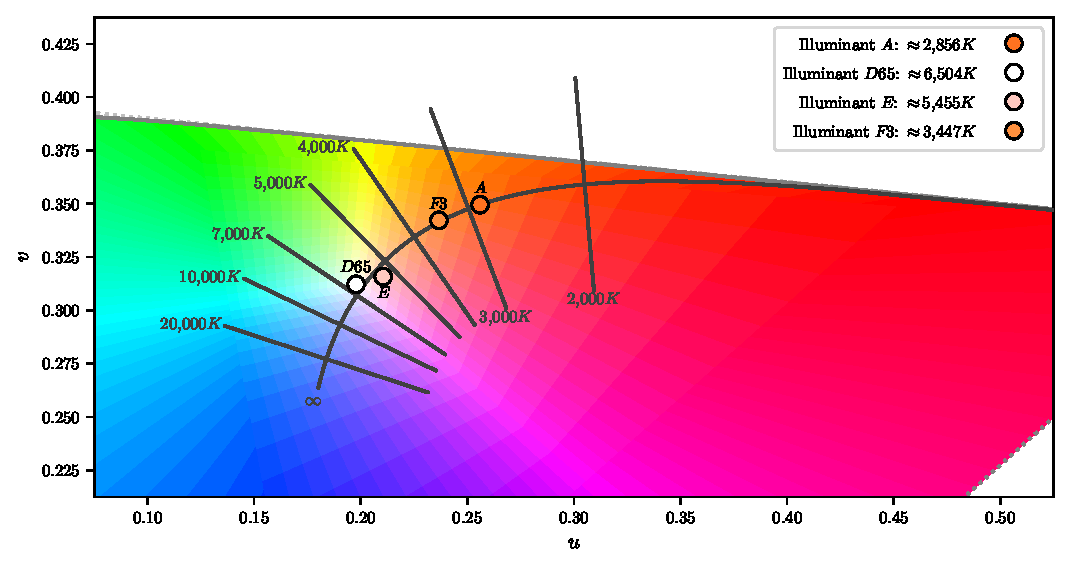
\includegraphics{../images/figure_22_isotherm_lines_zoom.pdf}
    \fi
    \caption{CIE 1960 $(u,v)$ chromaticity (zoomed in) showing isotherm lines for selected temperatures along the Planckian locus and standard illuminants $A$, $D65$, $E$, and $F3$.  IMAGE LINK, CODE LINK}\label{fig:isotherm_lines_zoom}
\end{figure*}

\begin{halffigure} % Figure 23
    \ifinvert
        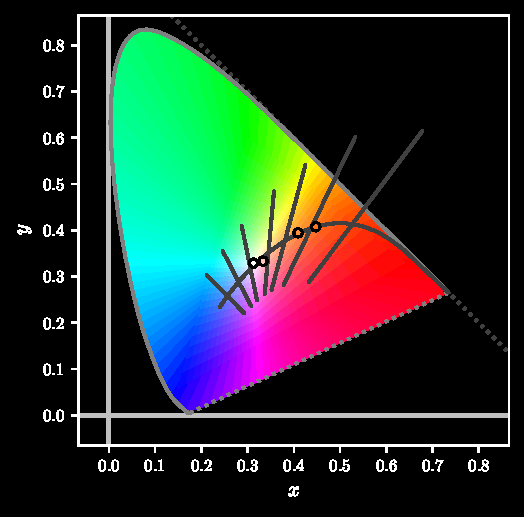
\includegraphics{../images/figure_23_cie_1931_isotherm_inverted.pdf}
    \else
        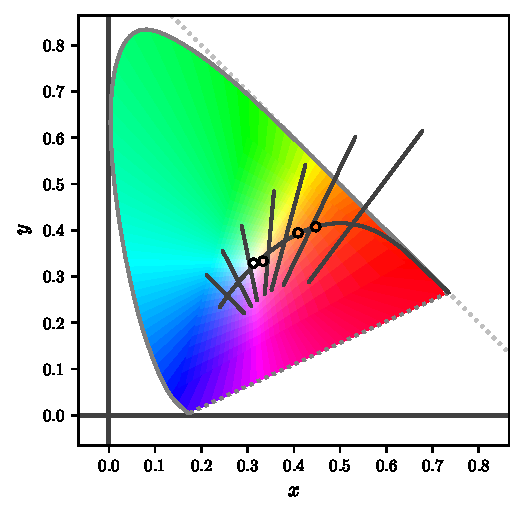
\includegraphics{../images/figure_23_cie_1931_isotherm.pdf}
    \fi
    \captionof{figure}{CIE 1931 $(x,y)$ chromaticity showing the same isotherm lines and standard illuminants as in Figure \ref{fig:isotherm_lines_zoom}.  Note that isotherm lines are not perpendicular to the Planckian locus and have varying lengths.  IMAGE LINK, CODE LINK}\label{fig:cie_1931_isotherm}
\end{halffigure}

Figure \ref{fig:cie_1931_isotherm} shows the same set of isotherm lines and standard illuminants in CIE 1931 $(x,y)$ chromaticity.  Note that the isotherm lines are not necessarily perpendicular and they do not have uniform length; therefore it is always necessary to estimate correlated color temperature within the CIE 1960 $(u,v)$ space in which it is defined even when using a different space for visualization.

\subsection{Links} % 5.3

\begin{itemize}
    \item Wikipedia
    \begin{itemize}
        \item \href{https://en.wikipedia.org/wiki/Planckian_locus}{Planckian Locus}
        \item \href{https://en.wikipedia.org/wiki/Standard_illuminant}{CIE Standard Illuminants}
    \end{itemize}
    \item Figure Images
    \begin{itemize}
        \item FIGURE 20 LIGHT AND DARK SVG
        \item FIGURE 21 LIGHT AND DARK SVG
        \item FIGURE 22 LIGHT AND DARK SVG
        \item FIGURE 23 LIGHT AND DARK SVG
    \end{itemize}
    \item GitHub Scripts
    \begin{itemize}
        \item FIGURE GENERATION FOR ALL FIGURES (20-23)
    \end{itemize}
\end{itemize}

\end{multicols}

% ================ SECTION 6 ================

\begin{figure*} % Figure 24
    \ifinvert
        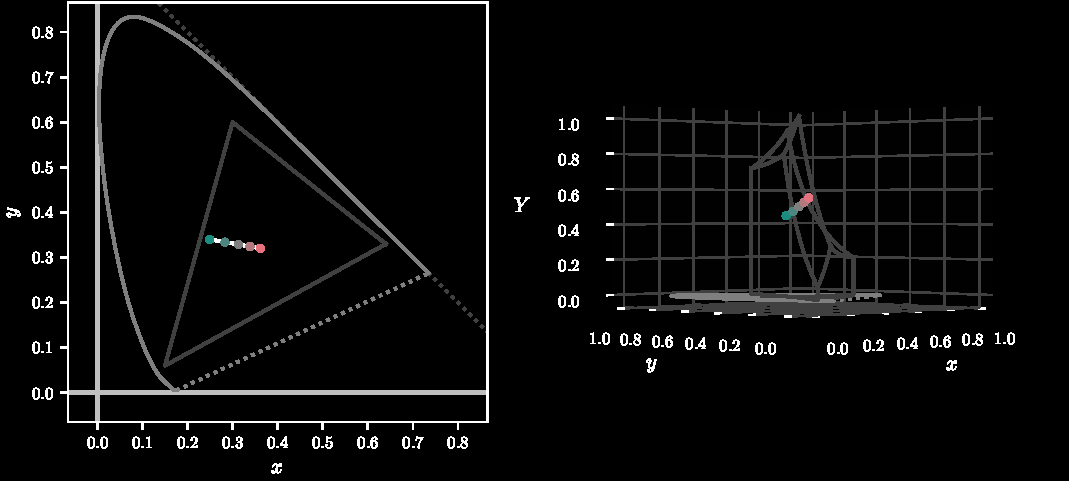
\includegraphics{../images/figure_24_single_protan_inverted.pdf}
    \else
        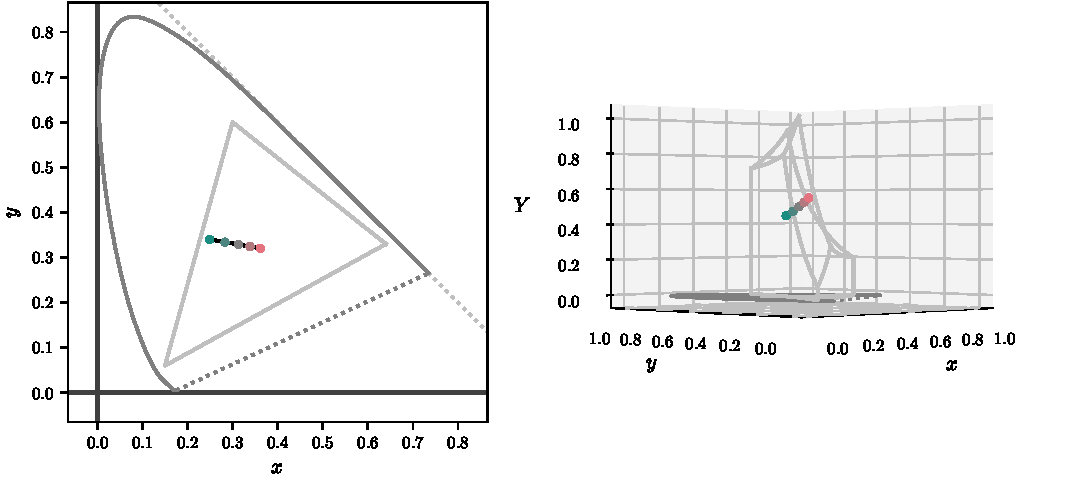
\includegraphics{../images/figure_24_single_protan.pdf}
    \fi
    \caption{The colors from Table \ref{table:varying_l_cone_activation} are plotted in chromaticity space (left) and chromoluminance space (right).  While the changes in long-wavelength-sensitive cone activation result in a straight line path in chromaticity, there are also changes in luminance that follow a slightly curved path.  IMAGE LINK, CODE LINK}\label{fig:single_protan}
\end{figure*}

\section{Color-Blindness} \label{sec:color_blindndess}

\begin{multicols}{2}

\begin{figure*} % Figure 25
    \ifinvert
        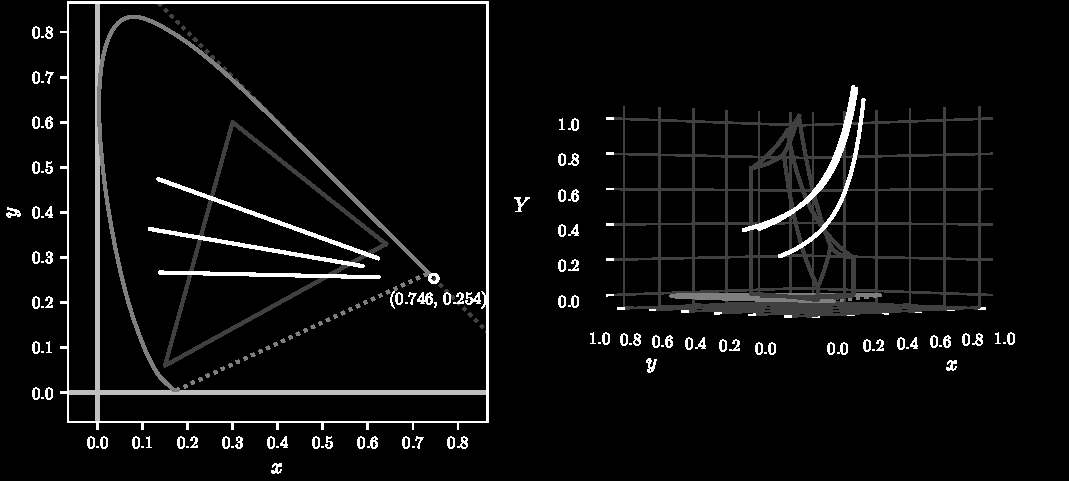
\includegraphics{../images/figure_25_multiple_protan_inverted.pdf}
    \else
        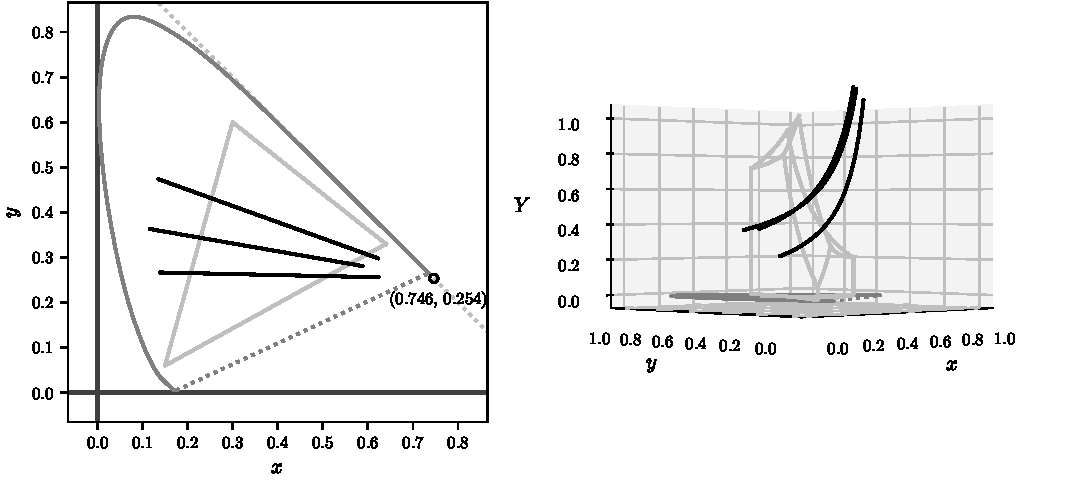
\includegraphics{../images/figure_25_multiple_protan.pdf}
    \fi
    \caption{Multiple protanope (missing long-wavelength-sensitive cone) confusion lines plotted in chromaticity (left) and chromoluminance (right).  The point where the chromaticity lines intersect - the copunctal point - is annotated in the left panel.  Note that in chromoluminance space the confusion line paths approach infinite luminance asymptotically as chromaticity goes toward the copunctal point.  IMAGE LINK, CODE LINK}\label{fig:multiple_protan}
\end{figure*}

\begin{figure*} % Figure 26
    \ifinvert
        \includegraphics{../images/figure_26_copunctal_points_inverted.pdf}
    \else
        \includegraphics{../images/figure_26_copunctal_points.pdf}
    \fi
    \caption{Select confusion lines converging on annotated copunctal points for (from left-to-right) the long-, medium-, and short-wavelength sensitive cones (protanope, deuteranope, and tritanope, respectively).  Horizontal bands of color each show a range of saturated colors whose chromaticities would be indistinguishable to someone missing that cone (though being saturated colors, luminance variation would be detectable).  IMAGE LINK, CODE LINK}\label{fig:copunctal_points}
\end{figure*}

\begin{figure*} % Figure 27
    \ifinvert
        \includegraphics{../images/figure_27_color_blind_stimuli_inverted.pdf}
    \else
        \includegraphics{../images/figure_27_color_blind_stimuli.pdf}
    \fi
    \caption{Example color-blind test stimuli for (from left-to-right) missing long-, medium-, or short-wavelength sensitive cones (protanope, deuteranope, and tritanope, respectively).  The object is to indicate the direction of the gap in the embedded "C" shape.  Below each stimulus is a chromaticity diagram showing the distribution of chromaticities in the stimulus (black fuzzy lines crossing the white point).  IMAGE LINK, CODE LINK}\label{fig:color_blind_stimuli}
\end{figure*}

Between the color matching experimental data of \cite{stiles1959npl} and the color matching functions of the CIE standard we transformed the data into cone sensitivity (the cone fundamentals).  The various linear transformations (and their inversions) allow us to convert any display red/green/blue triplet into a triplet of cone activations.  Knowing that a person with a missing cone photoreceptor type would be insensitive to changes in the nominal activation of that cone type, we can arbitrarily change the activation value for that cone and convert back to display red/green/blue.  The old and new display colors would not be distinguishable to the color-blind person.

\subsection{Confusion Lines \& Copunctal Points} % 6.1

Earlier we presented Equation \ref{eq:lms_to_xyz_10} to transform from cone fundamentals into color matching functions as part of our derivation of the CIE 170-2 10$^\circ$ standard.  Having switched to the CIE 1931 2$^\circ$ standard, we need a new transformation; starting in the opposite direction (\cite{smith1975spectral}):

\begin{equation} % Equation 30
    \begin{bmatrix}
        0.15514&0.54312&-0.03286\\
        -0.15514&0.45684&0.03286\\
        0&0&0.00801
    \end{bmatrix}\begin{bmatrix}
        X\\
        Y\\
        Z
    \end{bmatrix}=\begin{bmatrix}
        L\\
        M\\
        S
    \end{bmatrix}
\end{equation}

we can convert from color matching functions to cone fundamentals.  After manipulating one of the cone activations we can use the inverse transform to go back:

\begin{equation} % Equation 31
    \begin{bmatrix}
        2.94481&-3.50098&26.44303\\
        1.00004&1.00004&0\\
        0&0&124.84395
    \end{bmatrix}\begin{bmatrix}
        L\\
        M\\
        S
    \end{bmatrix}=\begin{bmatrix}
        X\\
        Y\\
        Z
    \end{bmatrix}
\end{equation}

As an explicit example, Table \ref{table:varying_l_cone_activation} provides the cone activation and display color values that result from arbitrarily manipulating the long-wavelength-sensitive cone activation value.  A person who lacks long-wavelength-sensitive cones should not see any chromaticity difference among the colors presented in the last column of the table (through they may detect differences in luminance).

\begin{halffigure} % Table 1
    \begin{tabular}{c|c|c|c|c|c|c}
        \hline
        $L$ & $M$ & $S$ & $R$ & $G$ & $B$\\
        \hline
        0.2783 & 0.1726 & 0.0044 & 0.1068 & 0.5480 & 0.5020 & \cellcolor{l1}\\
        0.3028 & 0.1726 & 0.0044 & 0.3034 & 0.5240 & 0.5010 & \cellcolor{l2}\\
        0.3274 & 0.1726 & 0.0044 & 0.5000 & 0.5000 & 0.5000 & \cellcolor{l3}\\
        0.3520 & 0.1726 & 0.0044 & 0.6966 & 0.4760 & 0.4990 & \cellcolor{l4}\\
        0.3765 & 0.1726 & 0.0044 & 0.8932 & 0.4520 & 0.4980 & \cellcolor{l5}
    \end{tabular}
    \captionof{table}{Varying the long-wavelength-sensitive cone activation ($L$ column) while holding the others constant and its effects on display color.}\label{table:varying_l_cone_activation}
\end{halffigure}

Plotting the chromaticity of the colors in Table \ref{table:varying_l_cone_activation} (see Figure \ref{fig:single_protan}) shows that they all fall in a straight line, however they do vary also in luminance and there the path is slightly curved.

Such lines drawn in chromaticity space where the activation of one cone type varies while the other two are fixed are called confusion lines for the cone type being varied.  A person who does not posses that cone type will not be able to discriminate chromaticity along any such line (but, again, there may be luminance changes to which they would still be sensitive).  Figure \ref{fig:multiple_protan} shows multiple, extended confusion lines for the long-wavelength-sensitive cones.

In chromaticity space the point where all confusion lines intersect (which invariably falls outside of the spectrum locus and the range of real spectra) is called the copunctal point.  Note that the luminances of the confusion paths in chromoluminance space approach infinity - an artifact of only modifying the cone activation of one cone type and not adjusting the other cones to maintain reasonable (let alone constant) luminance.  Using only the straight-line confusion lines in chromaticity space, and simply using previous methods to find the corresponding \textit{saturated} display color, Figure \ref{fig:copunctal_points} shows selected confusion lines for each of the cone types.

\subsection{Color-Blind Test Stimuli} % 6.2

Confusion lines pertain only to the discrimination of chromaticity and do not consider whether there are correlated luminances changes with chromaticity.  In fact, because our sensitivity to luminance differences is much better than our sensitivity to chromaticity changes, it is rather difficult to create visual stimuli that vary in chromaticity but are uniform in luminance (due to individual variability, stimuli must be adjusted to the individual observer \textit{and} their state of visual adaptation).  However, if an observer's task is to use chromaticity to identify the nature of some aspect of the stimulus, we can confound the ability to use luminance cues by causing luminance to vary randomly.  If there is no systematic correlation between chromaticity and luminance, then luminance information is useless for the task.

Figure \ref{fig:color_blind_stimuli} shows some example color-blind test stimuli.  The task would be for an observer to indicate whether the open gap in the embedded "C" is pointing up, right, down, or left.  The distribution of luminance among the constituent circles is random.  The distribution of chromaticity is bound to a confusion line for a particular cone type - so a person missing that cone type should see a field of uniform chromaticity and be unable to correctly identify the direction of the gap.

Beneath each test stimulus in Figure \ref{fig:color_blind_stimuli} is a chromaticity diagram showing the distribution of chromaticities present.  In this case all chromaticity distributions are taken from a confusion line passing through the white point, and the figure (the "C") chromaticities are taken from one side of white and the background chromaticities are taken from the opposite side of white.  In principle any confusion line will work for the purposes of such a color-blind test, and the two sides of the distribution need not be different hues, but it is easier to visualize in the way it is presented here.

The spread of the distribution of chromaticities can be varied to make the figure more or less difficult to discriminate. Finding the threshold beyond which an observer can no longer perform the task provides a measure of their sensitivity and a basis for judging whether one has a normal or below-normal sensitivity.  Figure \ref{fig:color_blind_stimuli_contrast} shows example color-blind stimuli of decreasing chromatic contrast from left-to-right.

\begin{figure*} % Figure 28
    \ifinvert
        \includegraphics{../images/figure_28_color_blind_stimuli_contrast_inverted.pdf}
    \else
        \includegraphics{../images/figure_28_color_blind_stimuli_contrast.pdf}
    \fi
    \caption{Color-blind test stimuli with decreasing contrast from left-to-right.  The distributions of chromaticities in the sample stimuli are taken from (from top-to-bottom) long-, medium-, and short-wavelength-sensitive confusion lines.  These stimuli are not calibrated - the reader should not take an ability or inability to perform the associated discrimination task here as an indication of whether or not they may be color-blind.  IMAGE LINK, CODE LINK}\label{fig:color_blind_stimuli_contrast}
\end{figure*}

\subsection{Color-Blind Filtered Images} % 6.3

It is common to illustrate the "effects" of color-blindness by filtering colorful images so as to remove chromatic contrast along confusion lines for a given missing cone type.  Figure \ref{fig:color_blind_filter_photograph} shows an example of such filtering (photograph \href{https://pixabay.com/photos/flower-field-flowers-field-trees-250016/}{source}).

\begin{figure*} % Figure 29
    \ifinvert
        \includegraphics{../images/figure_29_color_blind_filter_photograph_inverted.pdf}
    \else
        \includegraphics{../images/figure_29_color_blind_filter_photograph.pdf}
    \fi
    \caption{A colorful photograph filtered to remove chromatic differences to which an observer with a missing cone type would not be sensitive.  From left-to-right are the original image, a protanope filtered image, a deuteranope filtered image, and a tritanope filtered image.  Below each image is a chromaticity diagram showing the distribution of chromaticities in the image.  Note that the distributions of filtered images have an arc shape - the center around which the distribution arcs is the corresponding copunctal point for the missing cone type.  IMAGE LINK, CODE LINK}\label{fig:color_blind_filter_photograph}
\end{figure*}

There are some arbitrary choices made in the method for filtering illustrated in Figure \ref{fig:color_blind_filter_photograph}.  First, the filtering was accomplished by setting the chromatic distance from each associated copunctal point to be constant (hence the arc shaped lines along which the resulting chromaticities fall).  Second, that constant distance was chosen based on the average chromaticity of the original image - it could have just as easily been based on distance to the white point, here D65.  The result of these two arbitrary choices is that all of the images have more closely the same average chromaticity, but more importantly the two colors visible in each of the filtered images are purple/greenish-yellow, blue/yellow and pinkish-red/greenish-cyan for the three cone types.  This does not mean that color-blind people see these particular hues.  Figure \ref{fig:color_blind_filter_stimulus} shows the same filtering applied to one of the color-blind test stimuli.

\begin{figure*} % Figure 30
    \ifinvert
        \includegraphics{../images/figure_30_color_blind_filter_stimulus_inverted.pdf}
    \else
        \includegraphics{../images/figure_30_color_blind_filter_stimulus.pdf}
    \fi
    \caption{A color-blind test stimulus (protanope) filtered to remove chromatic differences to which an observer with a missing cone type would not be sensitive.  From left-to-right are the original image, a protanope filtered image, a deuteranope filtered image, and a tritanope filtered image.  Below each image is a chromaticity diagram showing the distribution of chromaticities in the image.  Note that in the second image from the left (filtered to mimic the chromatic discriminability of a protanope) the "C" figure is invisible (the distribution is a more-or-less uniform point).  IMAGE LINK, CODE LINK}\label{fig:color_blind_filter_stimulus}
\end{figure*}

\subsection{Links} % 6.4

\begin{itemize}
    \item Photograph \href{https://pixabay.com/photos/flower-field-flowers-field-trees-250016/}{source}
    \item Figure Images
    \begin{itemize}
        \item FIGURE 24 LIGHT AND DARK SVG
        \item FIGURE 25 LIGHT AND DARK SVG
        \item FIGURE 26 LIGHT AND DARK SVG
        \item FIGURE 27 LIGHT AND DARK SVG
        \item FIGURE 28 LIGHT AND DARK SVG
        \item FIGURE 29 LIGHT AND DARK SVG
        \item FIGURE 30 LIGHT AND DARK SVG
    \end{itemize}
    \item GitHub Scripts
    \begin{itemize}
        \item FIGURE GENERATION FOR ALL FIGURES (24-30)
    \end{itemize}
\end{itemize}

\end{multicols}

% ================ REFERENCES ================

\printbibliography


\end{document}